% !TeX encoding = UTF-8
%%%%%%%%%%%%%%%%%%%%%
%%%%% Anpassen! %%%%%
%%%%%%%%%%%%%%%%%%%%%
% Meta-Informationen 
\newcommand{\titel}{Community-basierte Wissensportale InDeKo.Navi Atlas}



\newcommand{\art}{Ausarbeitung}

\newcommand{\studiengang}{Wirtschaftsinformatik}

\newcommand{\autor}{Stephan Mende, Friederike Lauterbach, Konstantin Janzen, Robin Helmedach}

\newcommand{\email}{}

\newcommand{\matnr}{}

\newcommand{\institut}{Institut für Betriebswirtschaft und Wirtschaftsinformatik}

\newcommand{\arbeitsgruppe}{Arbeitsgruppe Informationssysteme und Unternehmensmodellierung}

\newcommand{\universitaet}{Universität Hildesheim \textbullet  Universitätsplatz 1 \textbullet  D-31134 Hildesheim}

\newcommand{\adresse}{\arbeitsgruppe  \textbullet  \institut \\ \universitaet}

\newcommand{\version}{Version 1.0}

\newcommand{\veranstaltung}{IT-Studienprojekt Master \\SoSe 2016 - WiSe 2016/2017}

%%%%%%%%%%%%%%%%%%%%%%%%%%%%%%%%%%%%%%%%%%%%%
%% Diese Datei muss nicht angepasst werden %%
%%%%%%%%%%%%%%%%%%%%%%%%%%%%%%%%%%%%%%%%%%%%%
% v1.3
%Schriftgröße, ein- oder zweiseitig, Papierformat, Dokumententyp
\documentclass[12pt,oneside,a4paper,bibliography=totoc,listof=totoc,
	ngerman,
	parskip=half, % Abstand zwischen Absätzen (halbe Zeile)
	headings=normal, % Größe der Überschriften verkleinern
	]{scrartcl}

%Seitenränder
\usepackage[left=2cm,right=2cm,top=2.5cm,bottom=2.5cm]{geometry}

%Neue Deutsche Rechtschreibung und Umlaute
\usepackage[T1]{fontenc}
\usepackage[utf8]{inputenc}
\usepackage[ngerman]{babel}
\usepackage[babel,german=quotes]{csquotes}
\usepackage{lmodern}
\usepackage[right]{eurosym}

\usepackage{caption}
\usepackage{subcaption}

%Kopf- und Fußzeile
\usepackage{fancyhdr}
\pagestyle{fancy} 
\fancyhf{}


\usepackage{lastpage}

\usepackage{tabularx}
\newcolumntype{L}[1]{>{\raggedright\arraybackslash}p{#1}} % linksbündig mit Breitenangabe
\newcolumntype{C}[1]{>{\centering\arraybackslash}p{#1}} % zentriert mit Breitenangabe
\newcolumntype{R}[1]{>{\raggedleft\arraybackslash}p{#1}} % rechtsbündig mit Breitenangabe

%Kopfzeile links bzw. innen
%\fancyhead[L]{\name}

%Kopfzeile mittig
%\fancyhead[R]{\thepage}

%Kopfzeile rechts bzw. außen
%\fancyhead[L]{\rightmark}

%Fußzeile
%\cfoot{\thepage}

% Kopfzeile und Fußzeile einstellen
%\textsc{\lhead{\name, \matrikel}
%\chead{\veranstaltung\ \ubungsnr}
%\rhead{\today}
\cfoot{\thepage\ / \pageref*{LastPage}}

%Linie oben / unten
\renewcommand{\headrulewidth}{0pt}
%\renewcommand{\footrulewidth}{0.5pt}



%Hübbsche Schriften im PDF-Viewer
\usepackage{ae}
\usepackage{times}


\usepackage{booktabs}

\makeatletter
\@ifpackageloaded{tex4ht}{%
      \usepackage[dvips]{graphicx}
      \usepackage[tex4ht]{hyperref}
    }{%

% Brauchbare PDF-Links und Angaben im PDF-Header
% Graphiken
\usepackage[pdftex]{graphicx}
\usepackage[hyphens]{url}
\PassOptionsToPackage{hyphens}{url}
\usepackage[ %pdftex,
	raiselinks=true,%
	bookmarks=true,%
	colorlinks=true,% Gibt man keine gedruckte Version ab, sondern das PDF, sollte man erwägen diesesn Wert auf "true" zu ändern
	linkcolor=black, % einfache interne Verknüpfungen
	anchorcolor=black, % Ankertext
	citecolor=black, % Verweise auf Literaturverzeichniseinträge im Text
	filecolor=black, % Verknüpfungen, die lokale Dateien öffnen
	menucolor=black, % Acrobat-Menüpunkte
	urlcolor=blue, 
	bookmarksopenlevel=1,%
	bookmarksopen=true,%
	bookmarksnumbered=true,%
	hyperindex=true,% 
	hypertexnames=false, % zur korrekten Erstellung der Bookmarks
	plainpages=false,% correct hyperlinks
	pdfpagelabels=true,% view TeX pagenumber in PDF reader
%%  pdfborder={0 0 0.5}
	pdfauthor={\autor},
	pdfsubject={\titel},
	pdfkeywords={},
	pdftitle={\titel},
	linktocpage = false, % Seitenzahlen anstatt Text im Inhaltsverzeichnis verlinken
	pdfstartview=FitH
]{hyperref}

}
\makeatother
%Thumbnails im PDF
%\usepackage{thumbpdf}
%hübschere Tabellenabstände
\usepackage{booktabs}

%diverser mathematischer Kram
\usepackage{amsmath}
\usepackage{amsthm}
\usepackage{amssymb}
\usepackage{multirow}

% Zitierstil
%\usepackage[round]{natbib}
%\usepackage[backend=biber, style=mla]{biblatex}
%\usepackage[backend=biber, style=apa]{biblatex}
%\usepackage[style=authoryear,natbib=true]{biblatex}
\usepackage[style=authoryear, maxnames=2, maxbibnames=99, backend=biber,firstinits=true, hyperref=true]{biblatex}
\DeclareNameAlias{sortname}{last-first}
%\DeclareLanguageMapping{ngerman}{ngerman-apa}



% Verhindern von "Schusterjungen" und "Hurenkindern"
\clubpenalty = 10000
\widowpenalty = 10000
\displaywidowpenalty = 10000
\tolerance=500 %Zeilenumbruch

% Abkürzungsverzeichnis
\usepackage[dua]{acronym}

%  Paket um ToDos einzufügen
\usepackage{todonotes}

%Für farbige Links
\usepackage{color, colortbl}
\definecolor{javared}{rgb}{0.6,0,0} % for strings
\definecolor{javagreen}{rgb}{0.25,0.5,0.35} % comments
\definecolor{javapurple}{rgb}{0.5,0,0.35} % keywords
\definecolor{javadocblue}{rgb}{0.25,0.35,0.75} % javadoc


\usepackage{listings}
\lstset{% general command to set parameter(s) 
frame=top,frame=bottom,
breaklines=true,
%basicstyle=\sffamily\footnotesize, % print whole listing small 
basicstyle=\verbatim@font\footnotesize,
keywordstyle=\color{javapurple}\bfseries, % ubold black keywords 
identifierstyle=, % nothing happens 
commentstyle=\color{javagreen}, % green comments 
stringstyle=\color{javared}, % typewriter type for strings 
morecomment=[s][\color{javadocblue}]{/**}{*/},
showstringspaces=false, % no special string spaces 
numbers=none, 
numberstyle=\sffamily\footnotesize, 
stepnumber=1, 
numbersep=10pt, 
showspaces=false, 
showtabs=false,
float=htbp, 
numberbychapter=true,
morekeywords={}
%columns=fullflexible, % can copy&paste listings
%language=R
} 
\renewcommand\lstlistingname{Code}

\usepackage{makeidx}
%\usepackage{url}
\usepackage{setspace}
\setlength{\parindent}{0pt} % Wie weit einrücken nach Absatz


%\usepackage{ulem}
\usepackage{enumerate}


\title{\titel}
\author{\autor}
\date{\today}

%\renewcommand{\topfraction}{0.85}
%\renewcommand{\textfraction}{0.1}

% Abstand Bild-Bildunterschrift
\setlength{\abovecaptionskip}{5pt plus 0pt minus 2pt} % Chosen fairly arbitrarily
\setlength{\belowcaptionskip}{5pt plus 0pt minus 2pt} % Chosen fairly arbitrarily

\usepackage{watermark}
%\renewcommand\arraystretch{1.3}% More space between table rows (MyValue=1.0 is for standard spacing)
\usepackage{array}
\newcolumntype{C}[1]{>{\centering\arraybackslash}m{#1}}

% Subliminal refinements towards typographical perfection
\usepackage{microtype}

% Intelligent cross-referencing
\usepackage[ngerman,nameinlink]{cleveref}

% Grafiken \ Plots
\usepackage{pgfplots,pgfplotstable}
\pgfplotsset{compat=1.11}
%\usepackage{tikz}
\usetikzlibrary{patterns}
\usetikzlibrary{intersections}
\usetikzlibrary{spy}
\usepgfplotslibrary{fillbetween}

% Pseudocode
\usepackage{algorithm}
\usepackage{algorithmicx}
\usepackage{algpseudocode}
%\usepackage{algorithm2e}

\usepackage{watermark}

\usepackage[clearempty]{titlesec}
% Einstellen der Schriftgrößen der Überschriften
\titleformat{\chapter}[hang]{\LARGE\bfseries}{\thechapter\quad}{0pt}{}
\titleformat{\section}[hang]{\Large\bfseries}{\thesection\quad}{0pt}{}
\titleformat{\subsection}[hang]{\large\bfseries}{\thesubsection\quad}{0pt}{}
\titleformat{\subsubsection}[hang]{\normalsize}{\thesubsubsection\quad}{0pt}{}

% Einstellen der Abstände vor und nach den Überschriften
\titlespacing{\subsubsection}{0pt}{0pt}{-5pt}

\usepackage{float}
\usepackage{enumitem}
%\usepackage[toc]{glossaries}
\selectlanguage{ngerman}

\newcommand*{\quelle}[1]{\par\raggedleft\scriptsize Quelle:~#1}
\DefineBibliographyStrings{german}{%
  andothers = {et al.},
}
%\addbibresource{atlas.bib}
\setlength\bibitemsep{5pt}  % Abstand zwischen 2 Einträgen im Verzeichnis

% Abstände von Listen
\setlist[itemize]{parsep=0pt, itemsep=5.0pt plus 2.0pt minus 1.0pt}
\setlist[enumerate]{parsep=0pt, itemsep=5.0pt plus 2.0pt minus 1.0pt}

% Zeilenabstand: 1.5
\onehalfspacing

% Zeilenabstand innerhalb von Tabellen
\renewcommand{\arraystretch}{1.2}

% Schriftart für URLs und Pfadangaben beibehalten (Pfadangaben kursiv)
\urlstyle{same}
\DeclareUrlCommand\path{\itshape\urlstyle{same}}

% Abstand nach Bildunterschrift
\captionsetup{belowskip=0pt}



%%%%%%%%%%%%%%%%%%%%%%%%%%%%%%%%%%%
%%%%% Hier geht der Text los! %%%%%
%%%%%%%%%%%%%%%%%%%%%%%%%%%%%%%%%%%
\begin{document}
\newcommand{\untertitel}{Überwachung und Steuerung der Entwicklung} 

%\bibliographystyle{plainnat}
%\bibliographystyle{alpha}
\pagenumbering{roman}

% Erzeugt das Deckblatt
%   Bei zu langem Arbeitstitel müssen die vertikalen Abstände (\vspace)
%   angepasst werden, damit das Deckblatt weiterhin auf eine Seite passt.
\begin{titlepage}
	\newgeometry{top=2cm,bottom=2cm,left=2cm,right=2cm}
	\begin{figure}
		\centering
		\begin{minipage}{0.28\textwidth}
			\begin{flushleft}
				
\includegraphics[scale=0.23]{csm_ISUM_Logo_Final_107dd2fa79.jpg}
			\end{flushleft}
		\end{minipage}
		\begin{minipage}{0.35\textwidth}
			\centering
			\hspace{0.25cm}
		\end{minipage}
		\begin{minipage}{0.25\textwidth}
			\begin{flushright}
				
\includegraphics[scale=0.25]{St_Uni-Logo-9-2003-eps-converted-to.pdf}
			\end{flushright}
		\end{minipage}
		\vspace{4cm}
	\end{figure}
	\begin{center}
		
		\Huge{\textbf{\titel}}
		
		\Huge{\textbf{\untertitel}}
		\vspace{2cm}
	\end{center}
	\begin{center}
		\vspace*{0cm}
		\textbf{Ausarbeitung im Rahmen der Veranstaltung \veranstaltung}
		\vspace{1cm}
	\end{center}
	\begin{center}
		Institut für Betriebswirtschaft und Wirtschaftsinformatik,
		
		\arbeitsgruppe
	\end{center}
	\begin{center}
		\vspace{4cm}
		\autor\\
		

		\today
	\end{center}
\end{titlepage}
\newpage

\newgeometry{left=2cm,right=2cm,top=2.5cm,bottom=2.5cm,includefoot,footskip=0.5cm}
% Erzeugt das Inhaltsverzeichnis
%\tableofcontents

% Erzeugt das Abbildungsverzeichnis
\newpage
\listoffigures
\listoftables

\newpage
\restoregeometry

\setlength{\belowcaptionskip}{0pt} % Chosen fairly arbitrarily
\setlength{\abovecaptionskip}{-60pt} % Chosen fairly arbitrarily

\pagenumbering{arabic}

\label{DailyScrum}
\pdfbookmark[1]{Daily Scrum Entwicklung}{DailyScrum}
\begin{landscape}
	\parbox[c][\textwidth][s]{\linewidth}{%
		\vfill
		\captionsetup{type=figure}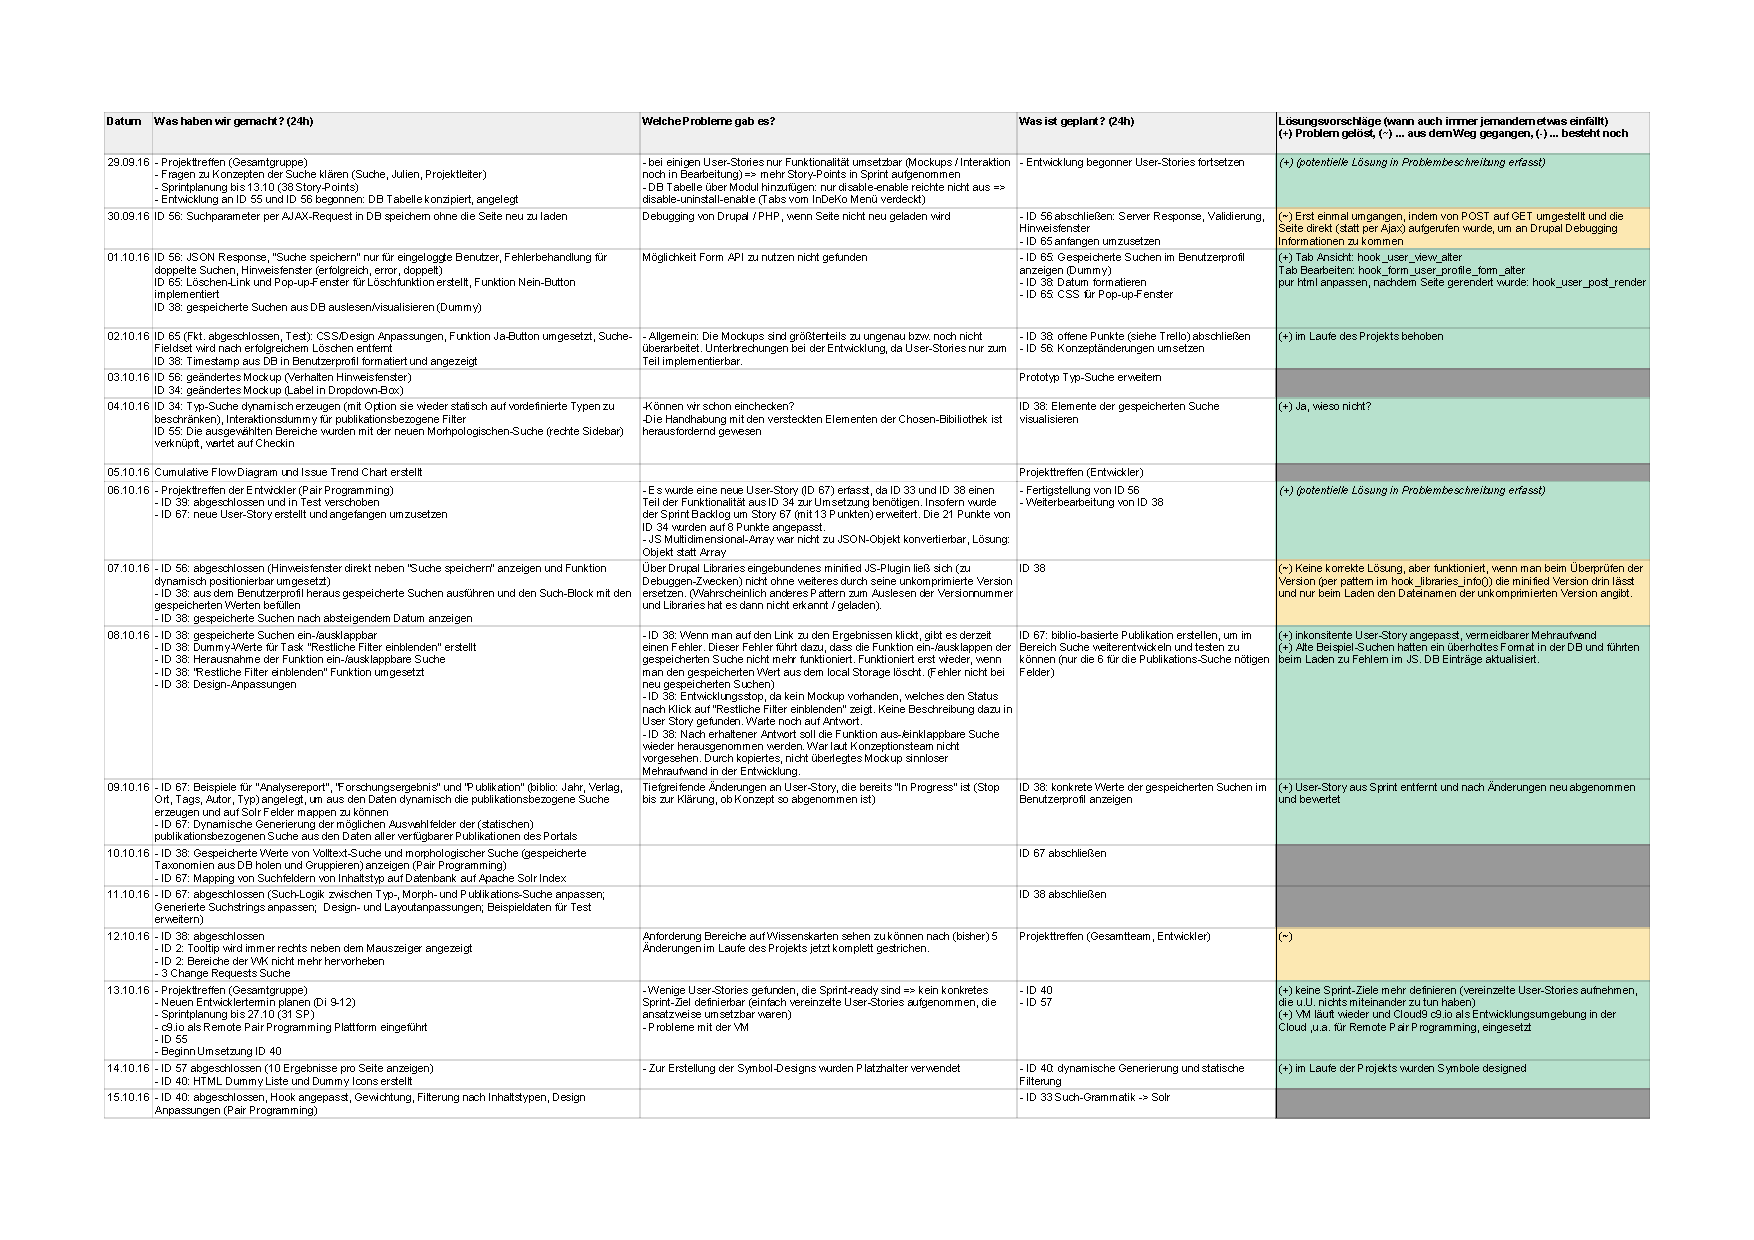
\includegraphics[page=1,width=\dimexpr\linewidth-2\fboxsep-2\fboxrule\relax]{daily}

		\vfill	
	}
	\captionof{table}{\textit{Daily Scrum} Entwicklung 29.09.2016 - 15.10.2016}
\end{landscape}

\begin{landscape}
	\parbox[c][\textwidth][s]{\linewidth}{%
		\vfill
		\captionsetup{type=figure}\includegraphics[page=2,width=\dimexpr\linewidth-2\fboxsep-2\fboxrule\relax]{daily}
		
		\vfill	
	}
	\captionof{table}{\textit{Daily Scrum} Entwicklung 16.10.2016 - 09.11.2016}
\end{landscape}

\begin{landscape}
	\parbox[c][\textwidth][s]{\linewidth}{%
		\vfill
		\captionsetup{type=figure}\includegraphics[page=3,width=\dimexpr\linewidth-2\fboxsep-2\fboxrule\relax]{daily}
		
		\vfill	
	}
	\captionof{table}{\textit{Daily Scrum} Entwicklung 10.11.2016 - 13.12.2016}
\end{landscape}

\begin{landscape}
	\parbox[c][\textwidth][s]{\linewidth}{%
		\vfill
		\captionsetup{type=figure}\includegraphics[page=4,width=\dimexpr\linewidth-2\fboxsep-2\fboxrule\relax]{daily}
		
		\vfill	
	}
	\captionof{table}{\textit{Daily Scrum} Entwicklung 14.12.2016 - 23.01.2017}
\end{landscape}

\begin{landscape}
	\parbox[c][\textwidth][s]{\linewidth}{%
		\vfill
		\captionsetup{type=figure}\includegraphics[page=5,width=\dimexpr\linewidth-2\fboxsep-2\fboxrule\relax]{daily}
		
		\vfill	
	}
	\captionof{table}{\textit{Daily Scrum} Entwicklung 24.01.2017 - 06.03.2017}
\end{landscape}
	
\begin{landscape}
	\parbox[c][\textwidth][s]{\linewidth}{%
		\vfill
		\captionsetup{type=figure}\includegraphics[page=6,width=\dimexpr\linewidth-2\fboxsep-2\fboxrule\relax]{daily}
		
		\vfill	
	}
	\captionof{table}{\textit{Daily Scrum} Entwicklung 07.03.2017 - 31.03.2017}
\end{landscape}








\label{burndown}
\pdfbookmark[1]{Burndown / Velocity Chart}{burndown}
\begin{landscape}
	\parbox[c][\textwidth][s]{\linewidth}{%
		\vfill
		\captionsetup{type=figure}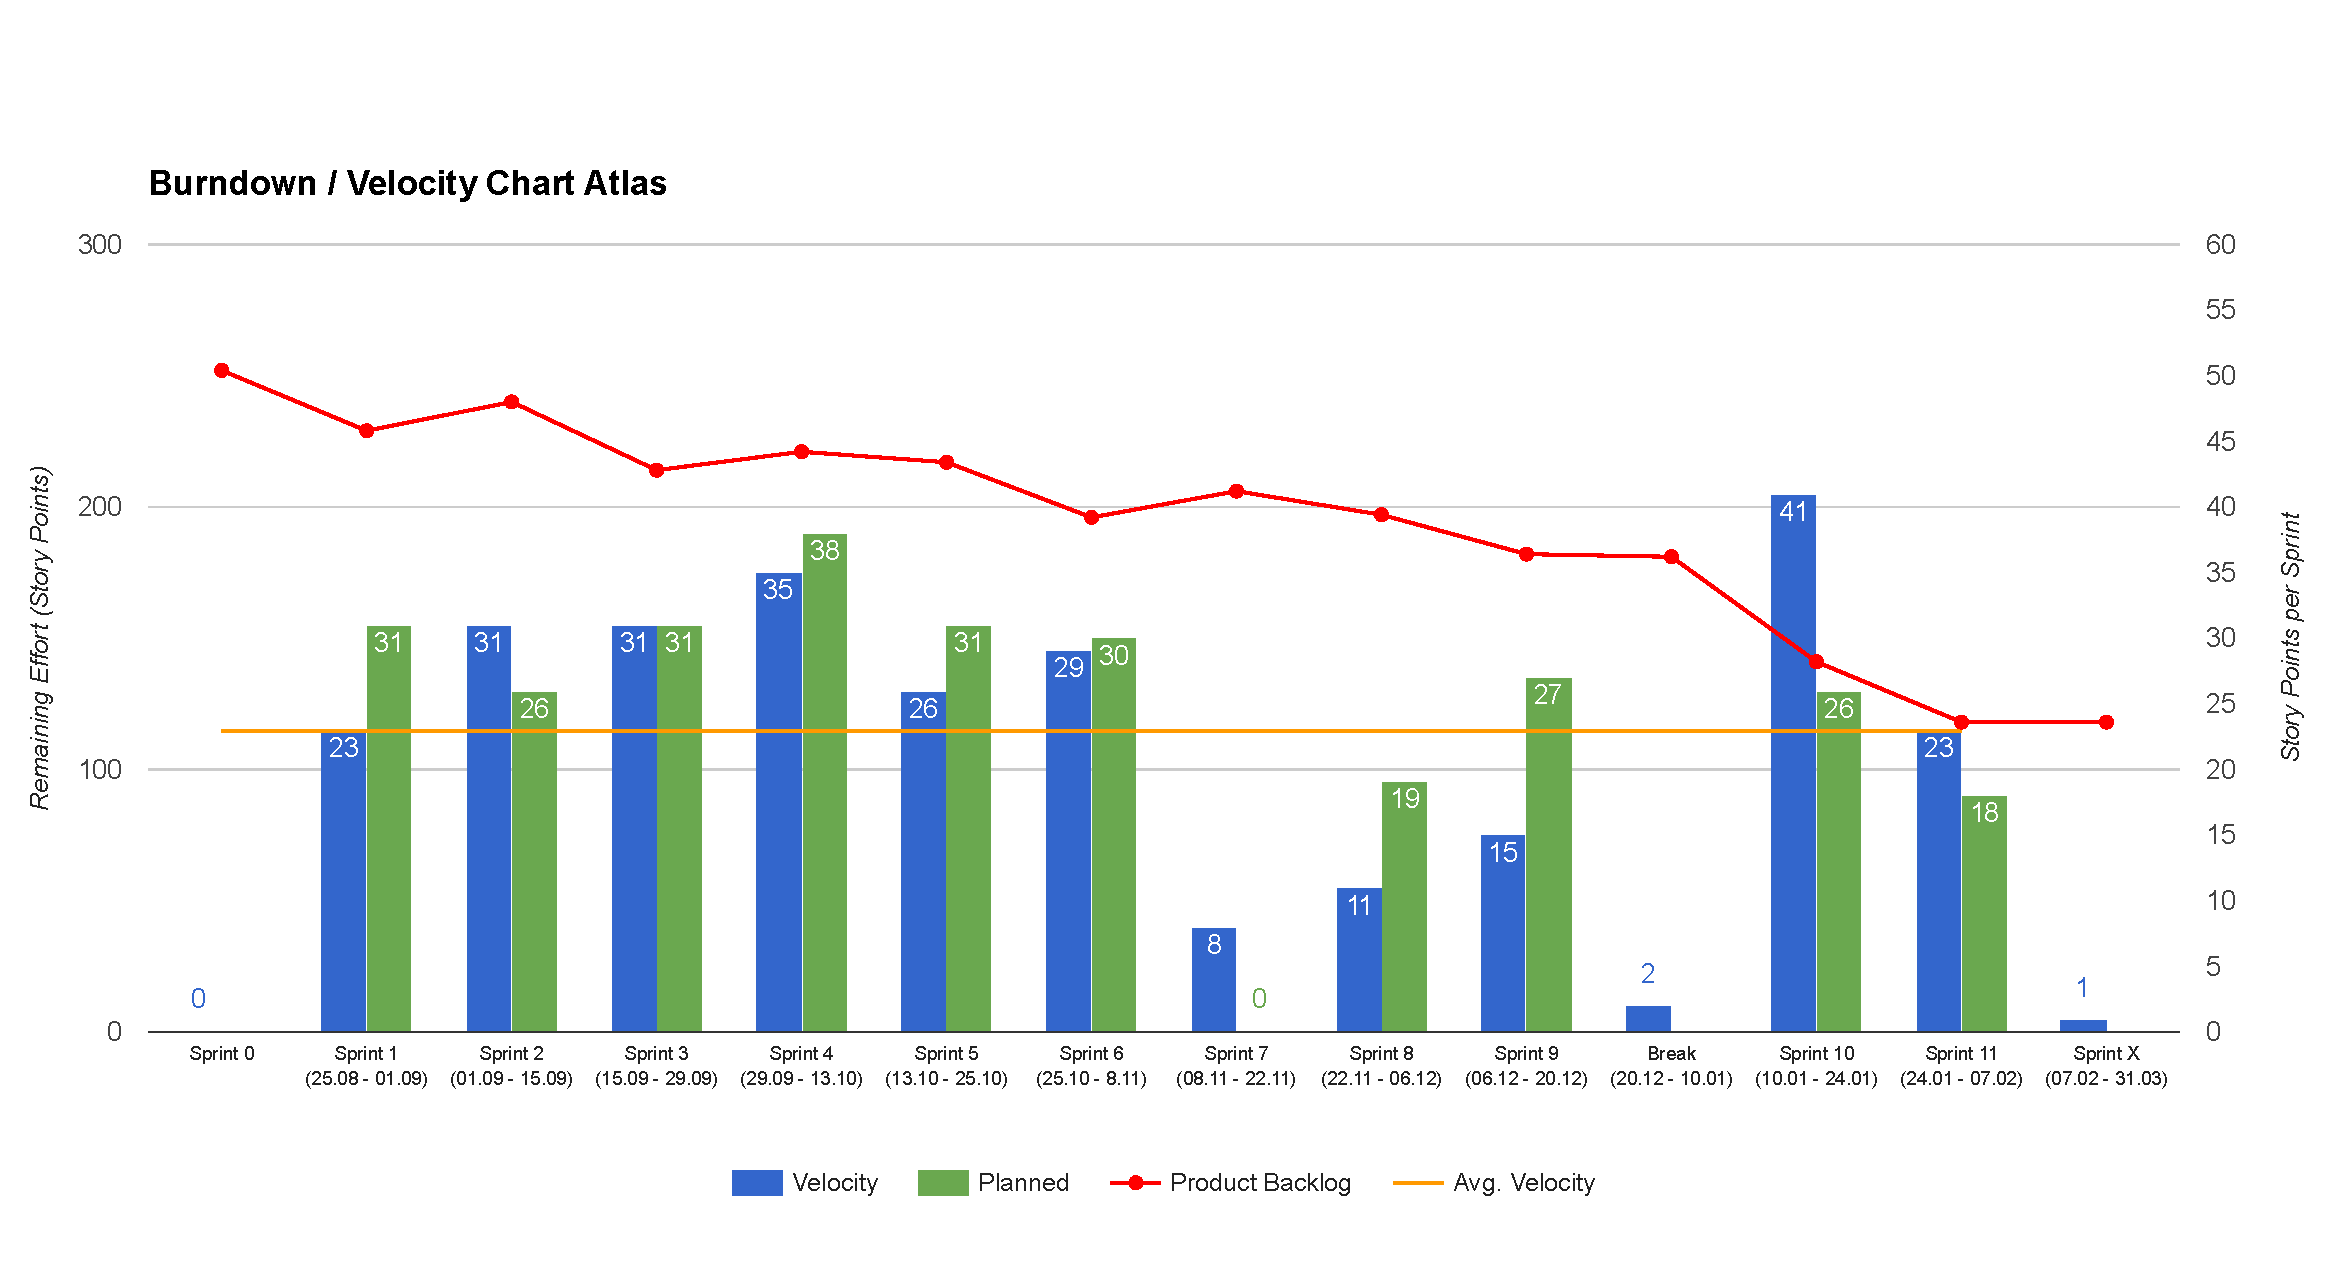
\includegraphics[page=1,width=\dimexpr\linewidth-2\fboxsep-2\fboxrule\relax]{svg/burndown}
		
		\vfill	
	}
	\captionof{figure}{\textit{Burndown / Velocity Chart}}
\end{landscape}




\label{cfd_sprint}
\pdfbookmark[1]{Cumulative Flow Diagram (Sprintphase)}{cfd_sprint}
\begin{landscape}
	\parbox[c][\textwidth][s]{\linewidth}{%
		\vfill
		\captionsetup{type=figure}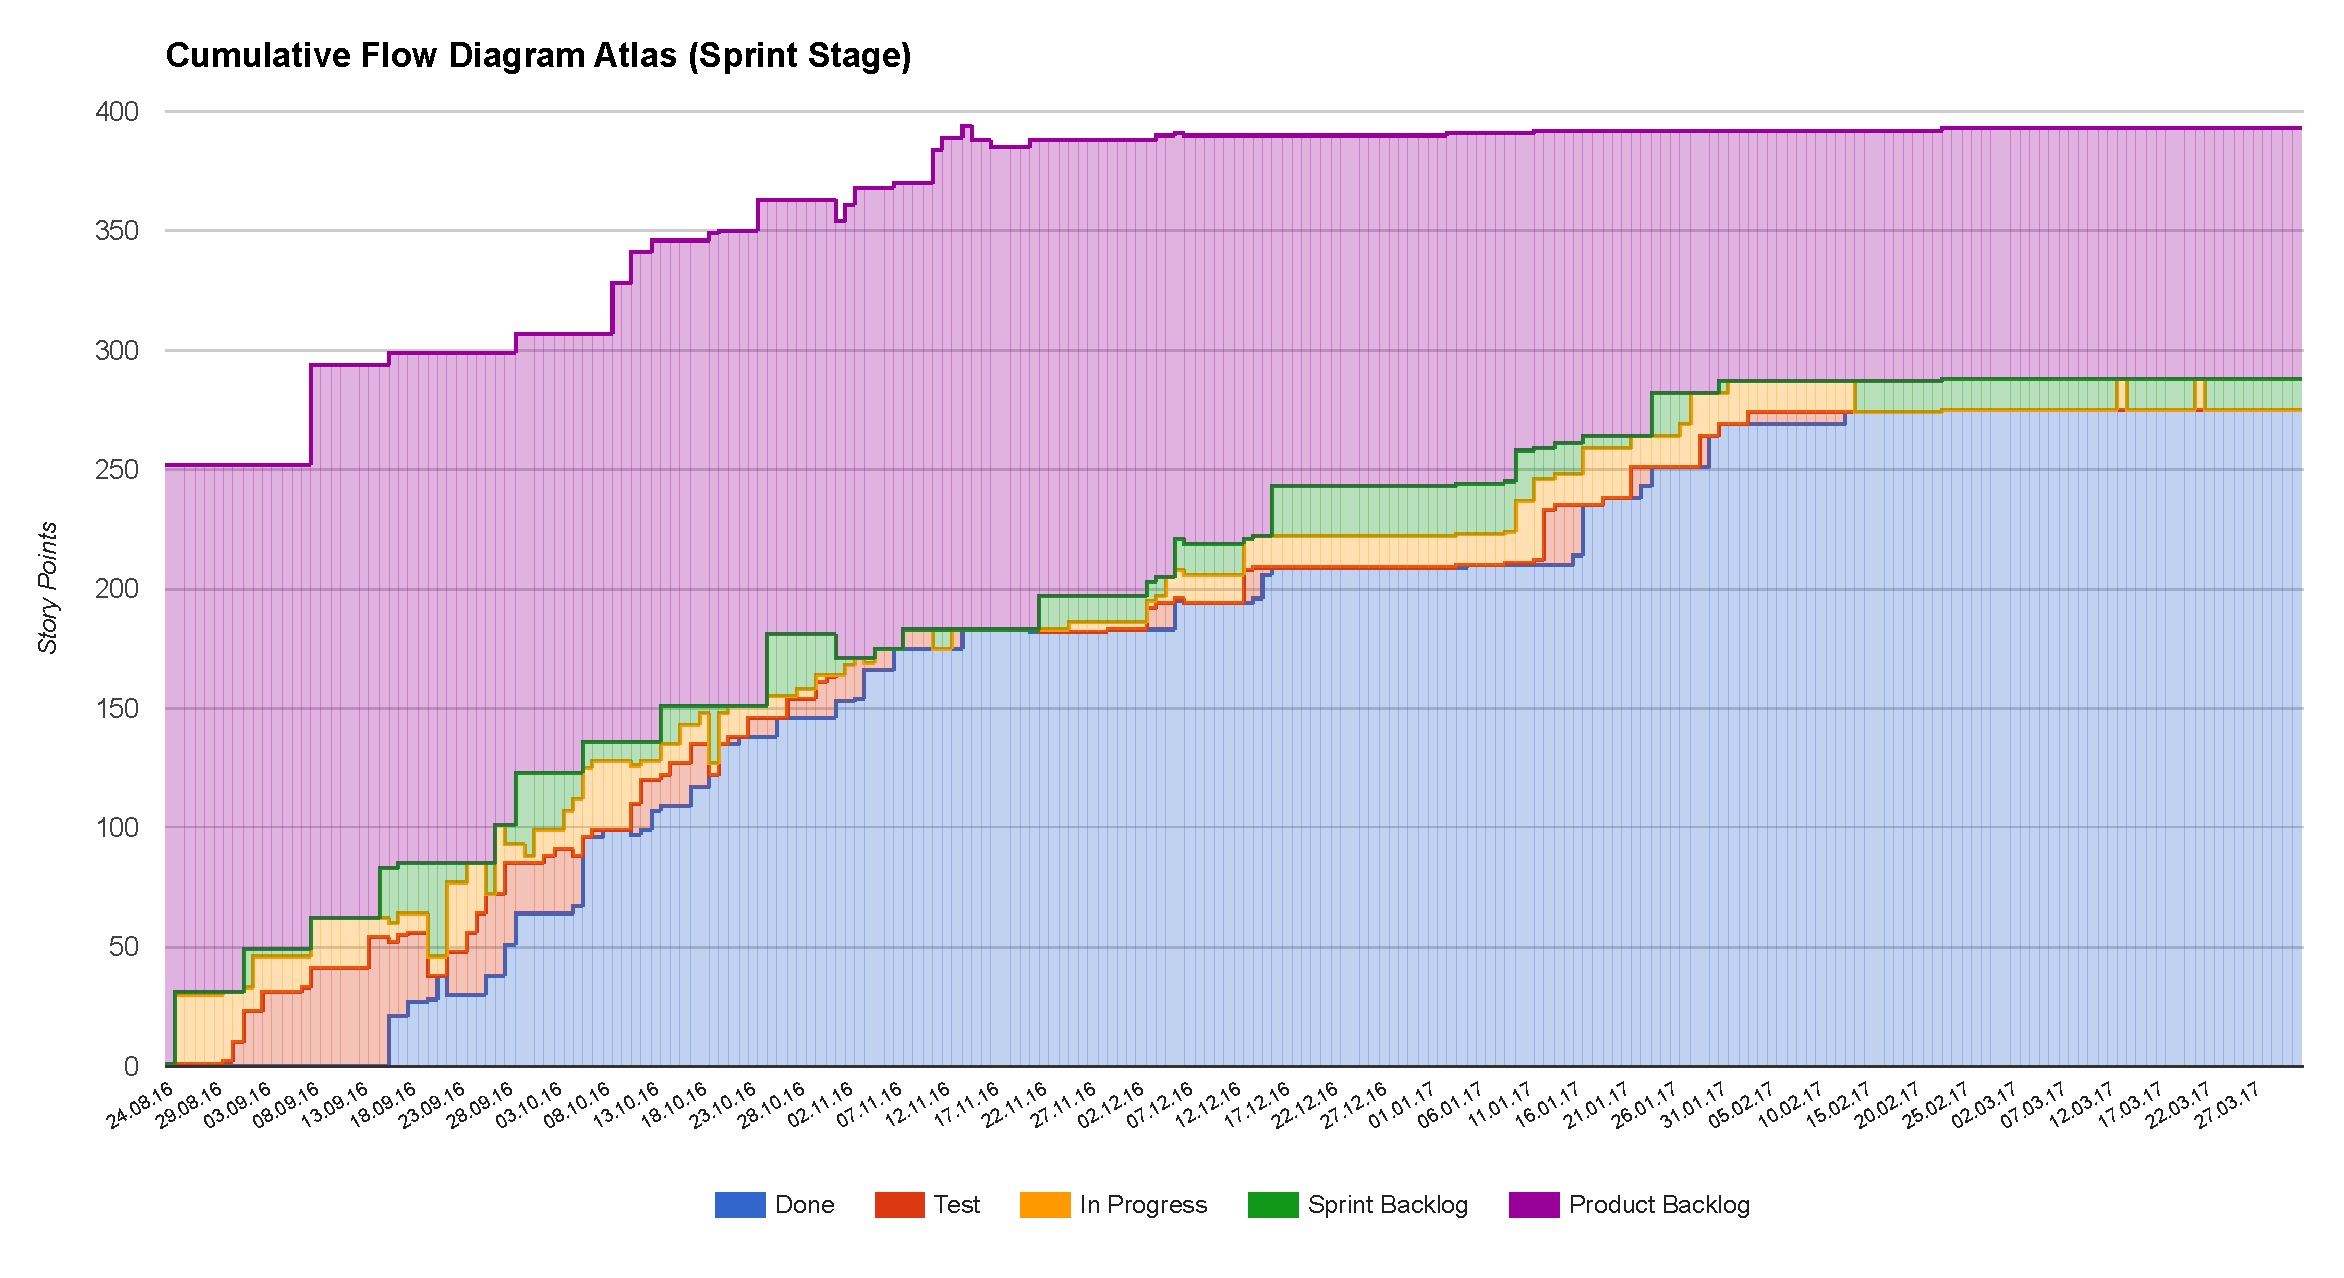
\includegraphics[page=1,width=\dimexpr\linewidth-2\fboxsep-2\fboxrule\relax]{svg/cfd_sprint}
		
		\vfill	
	}
	\captionof{figure}{\textit{Cumulative Flow Diagram} (Sprintphase)}
\end{landscape}




\label{issue}
\pdfbookmark[1]{Issue / Trend Chart}{issue}
\begin{landscape}
	\parbox[c][\textwidth][s]{\linewidth}{%
		\vfill
		\captionsetup{type=figure}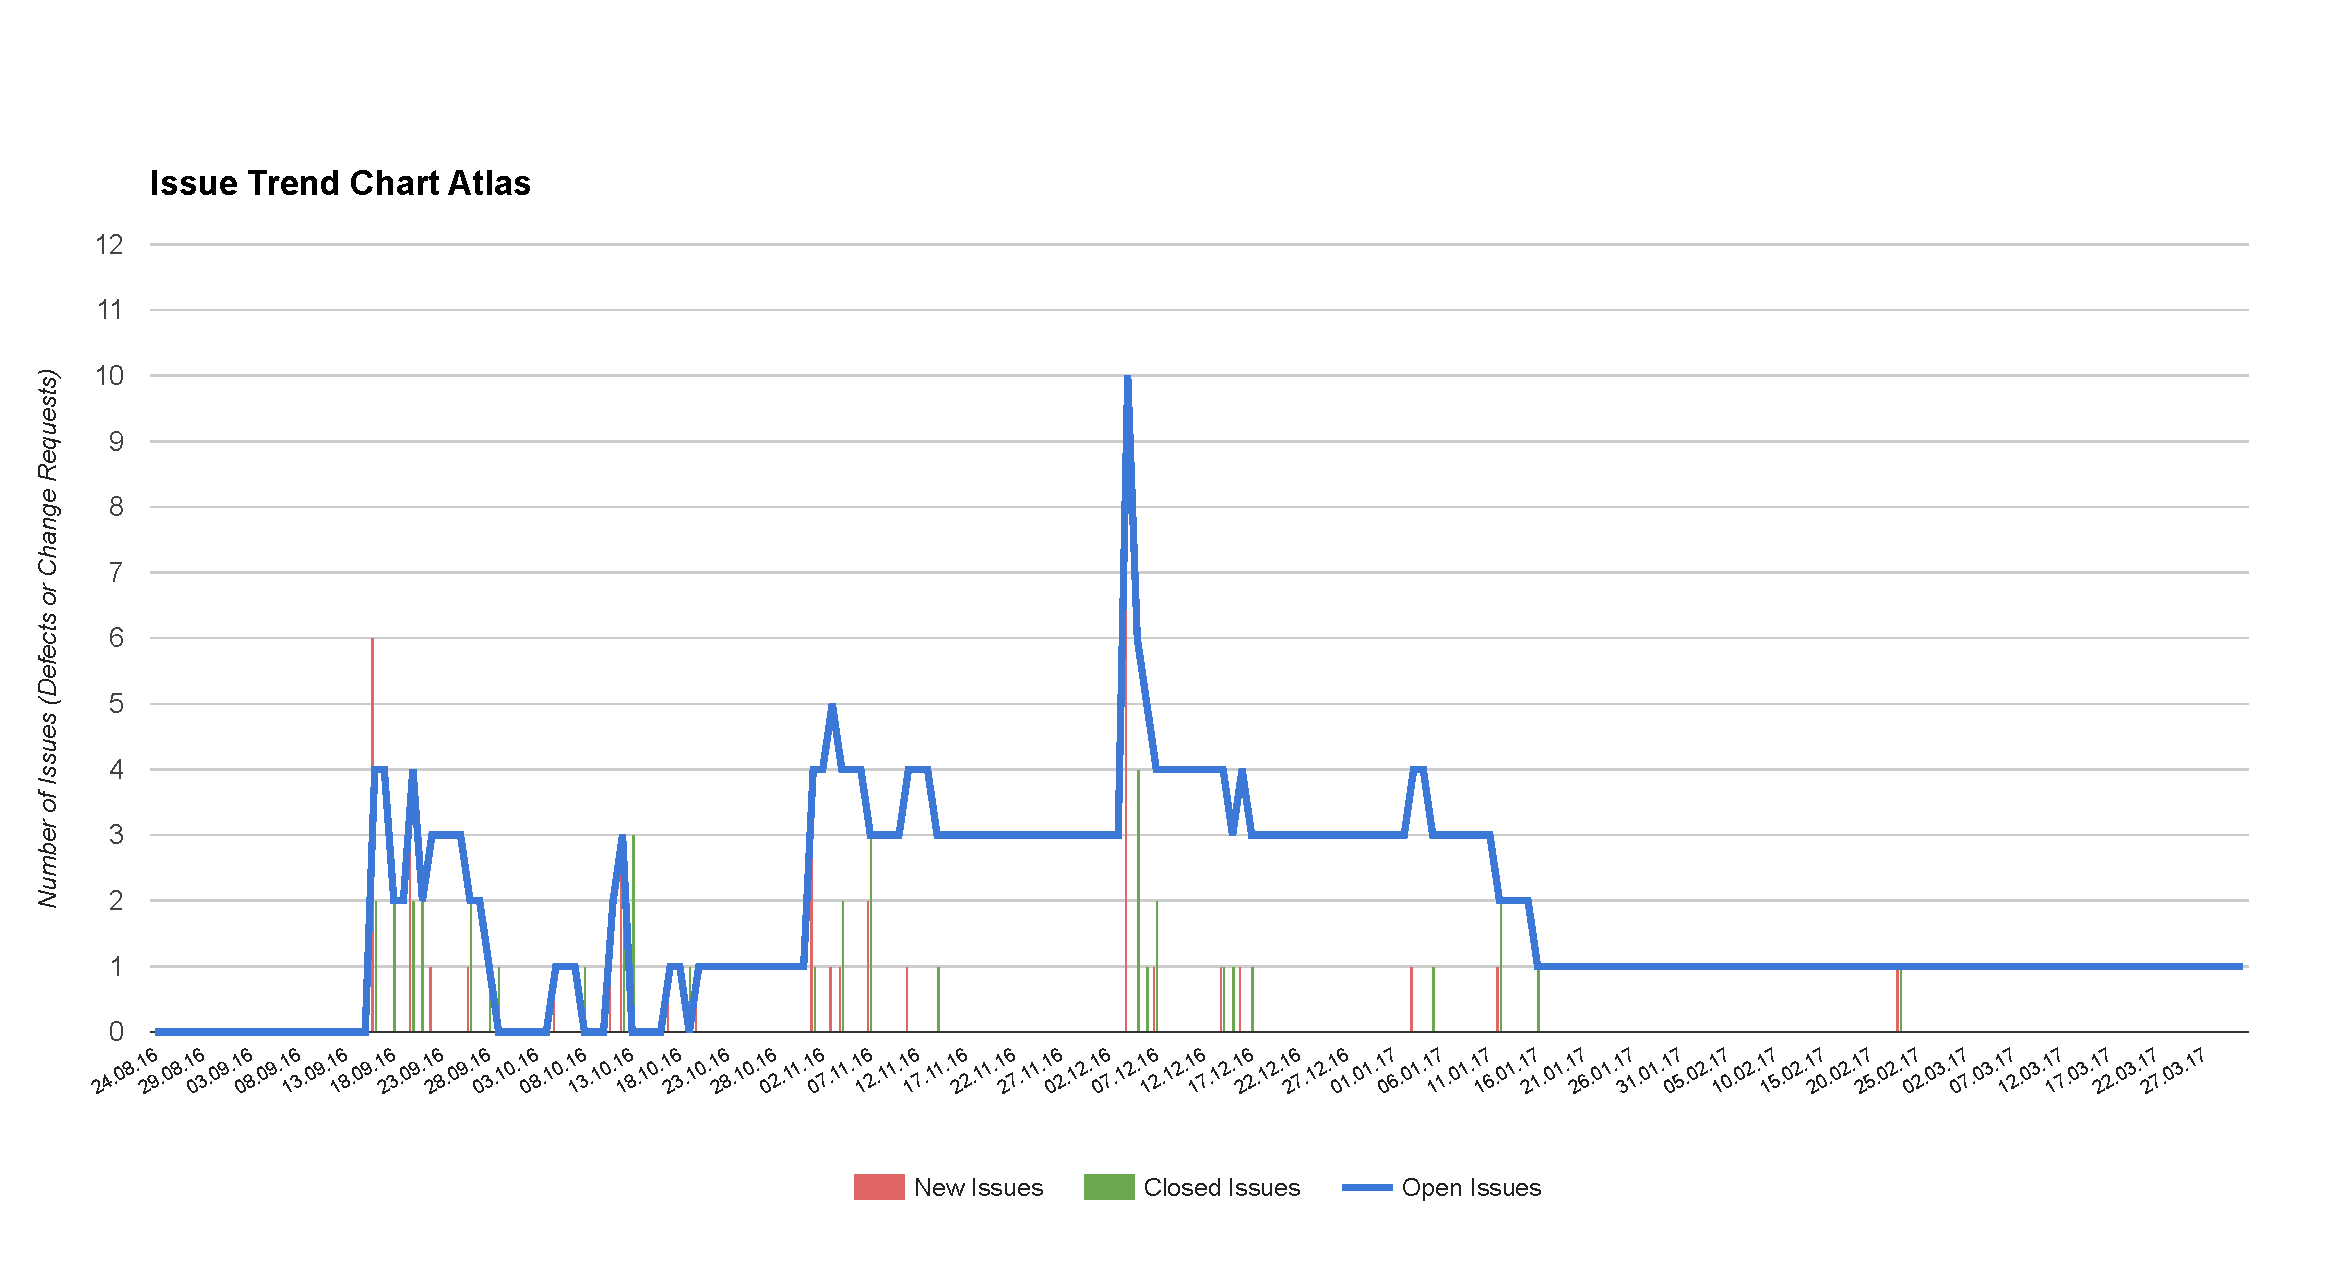
\includegraphics[page=1,width=\dimexpr\linewidth-2\fboxsep-2\fboxrule\relax]{svg/issue}
		
		\vfill	
	}
	\captionof{figure}{\textit{Issue / Trend Chart}}
\end{landscape}





\begin{figure}
	\label{pair}
	\pdfbookmark[1]{Pair Programming Matrix (Sprintphase)}{pair}
	\centering
	\captionsetup{type=figure}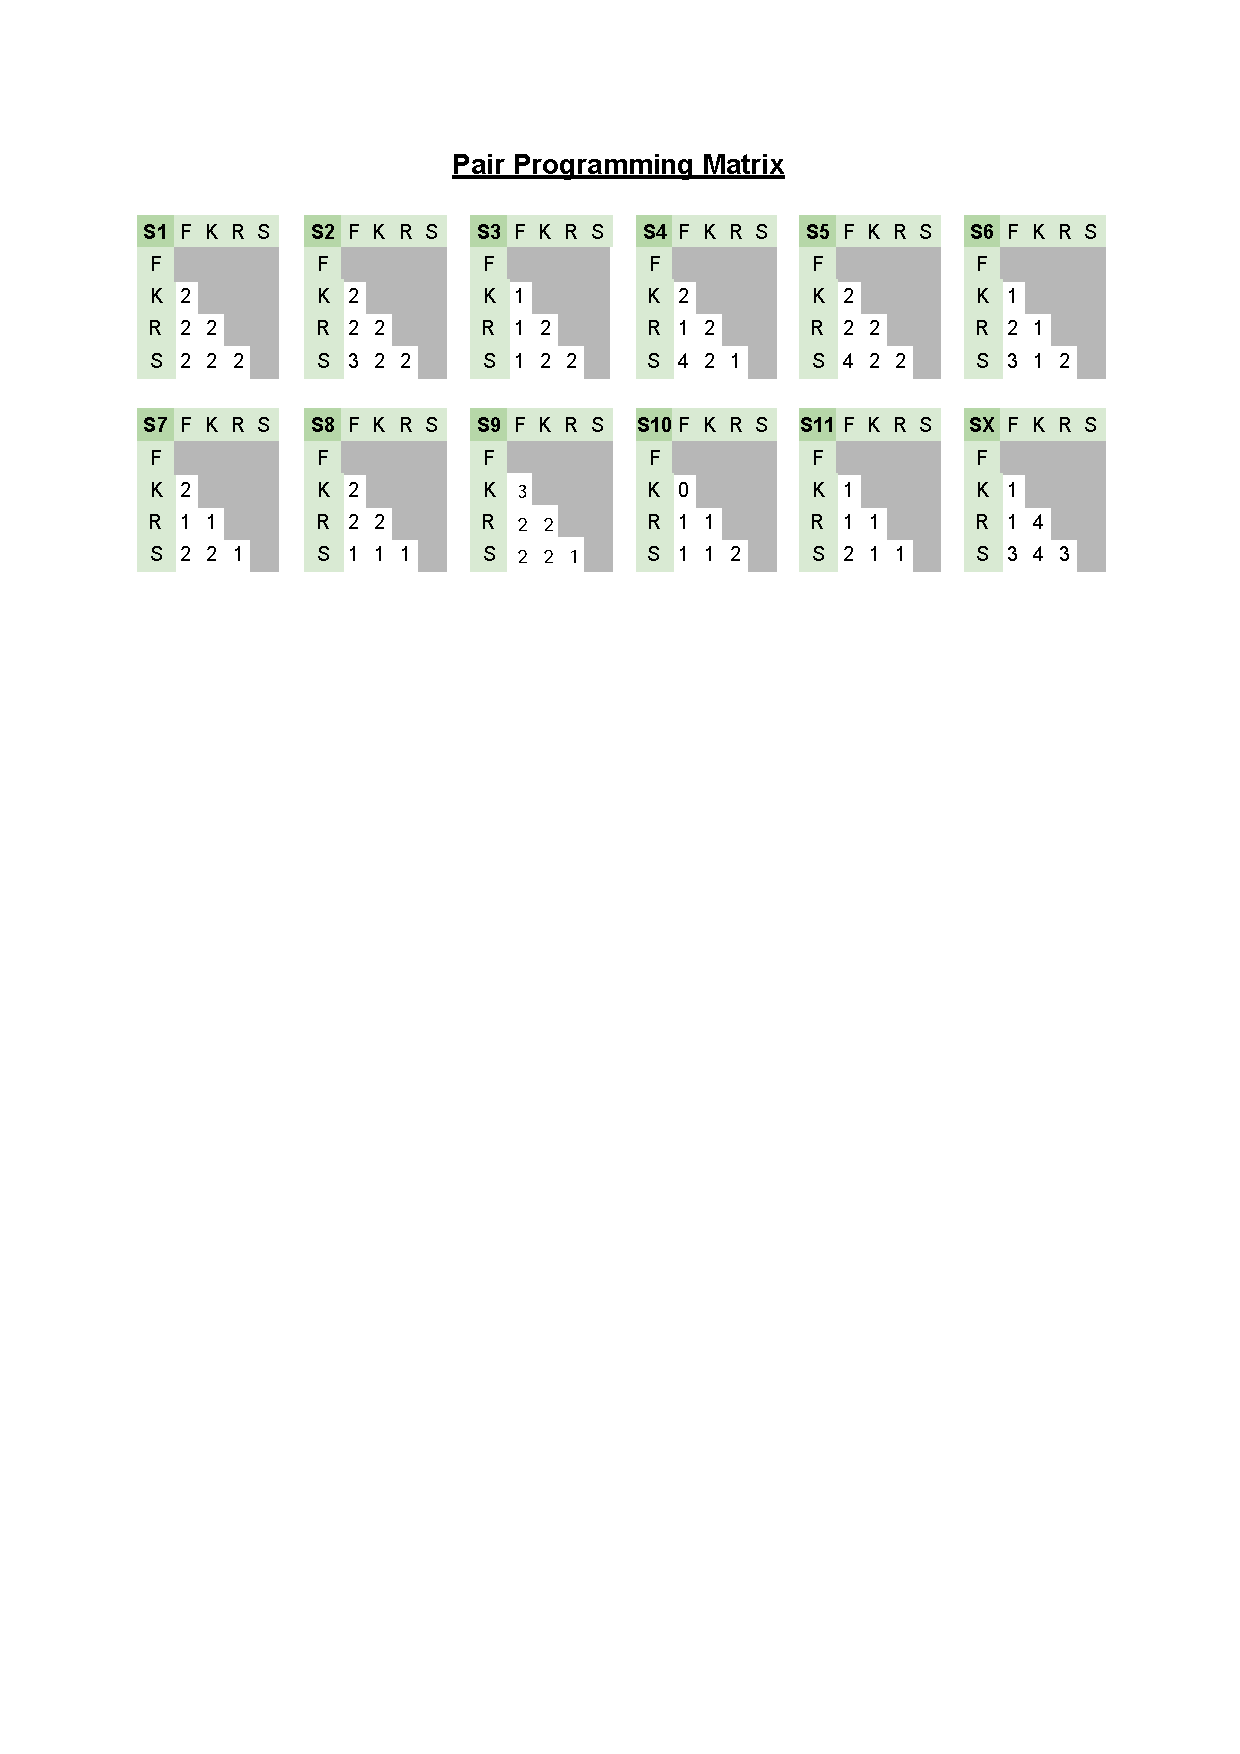
\includegraphics[page=1,width=\linewidth]{pair}
	
	\vspace{-17.3cm}
	\captionof{table}{\textit{Pair Programming Matrix} (Sprintphase)}
\end{figure}







\label{cfd_all}
\pdfbookmark[1]{Cumulative Flow Diagram mit Meilensteinen (Gesamtes Projekt)}{cfd_all}
\begin{landscape}
	\parbox[c][\textwidth][s]{\linewidth}{%
		\vfill
		\captionsetup{type=figure}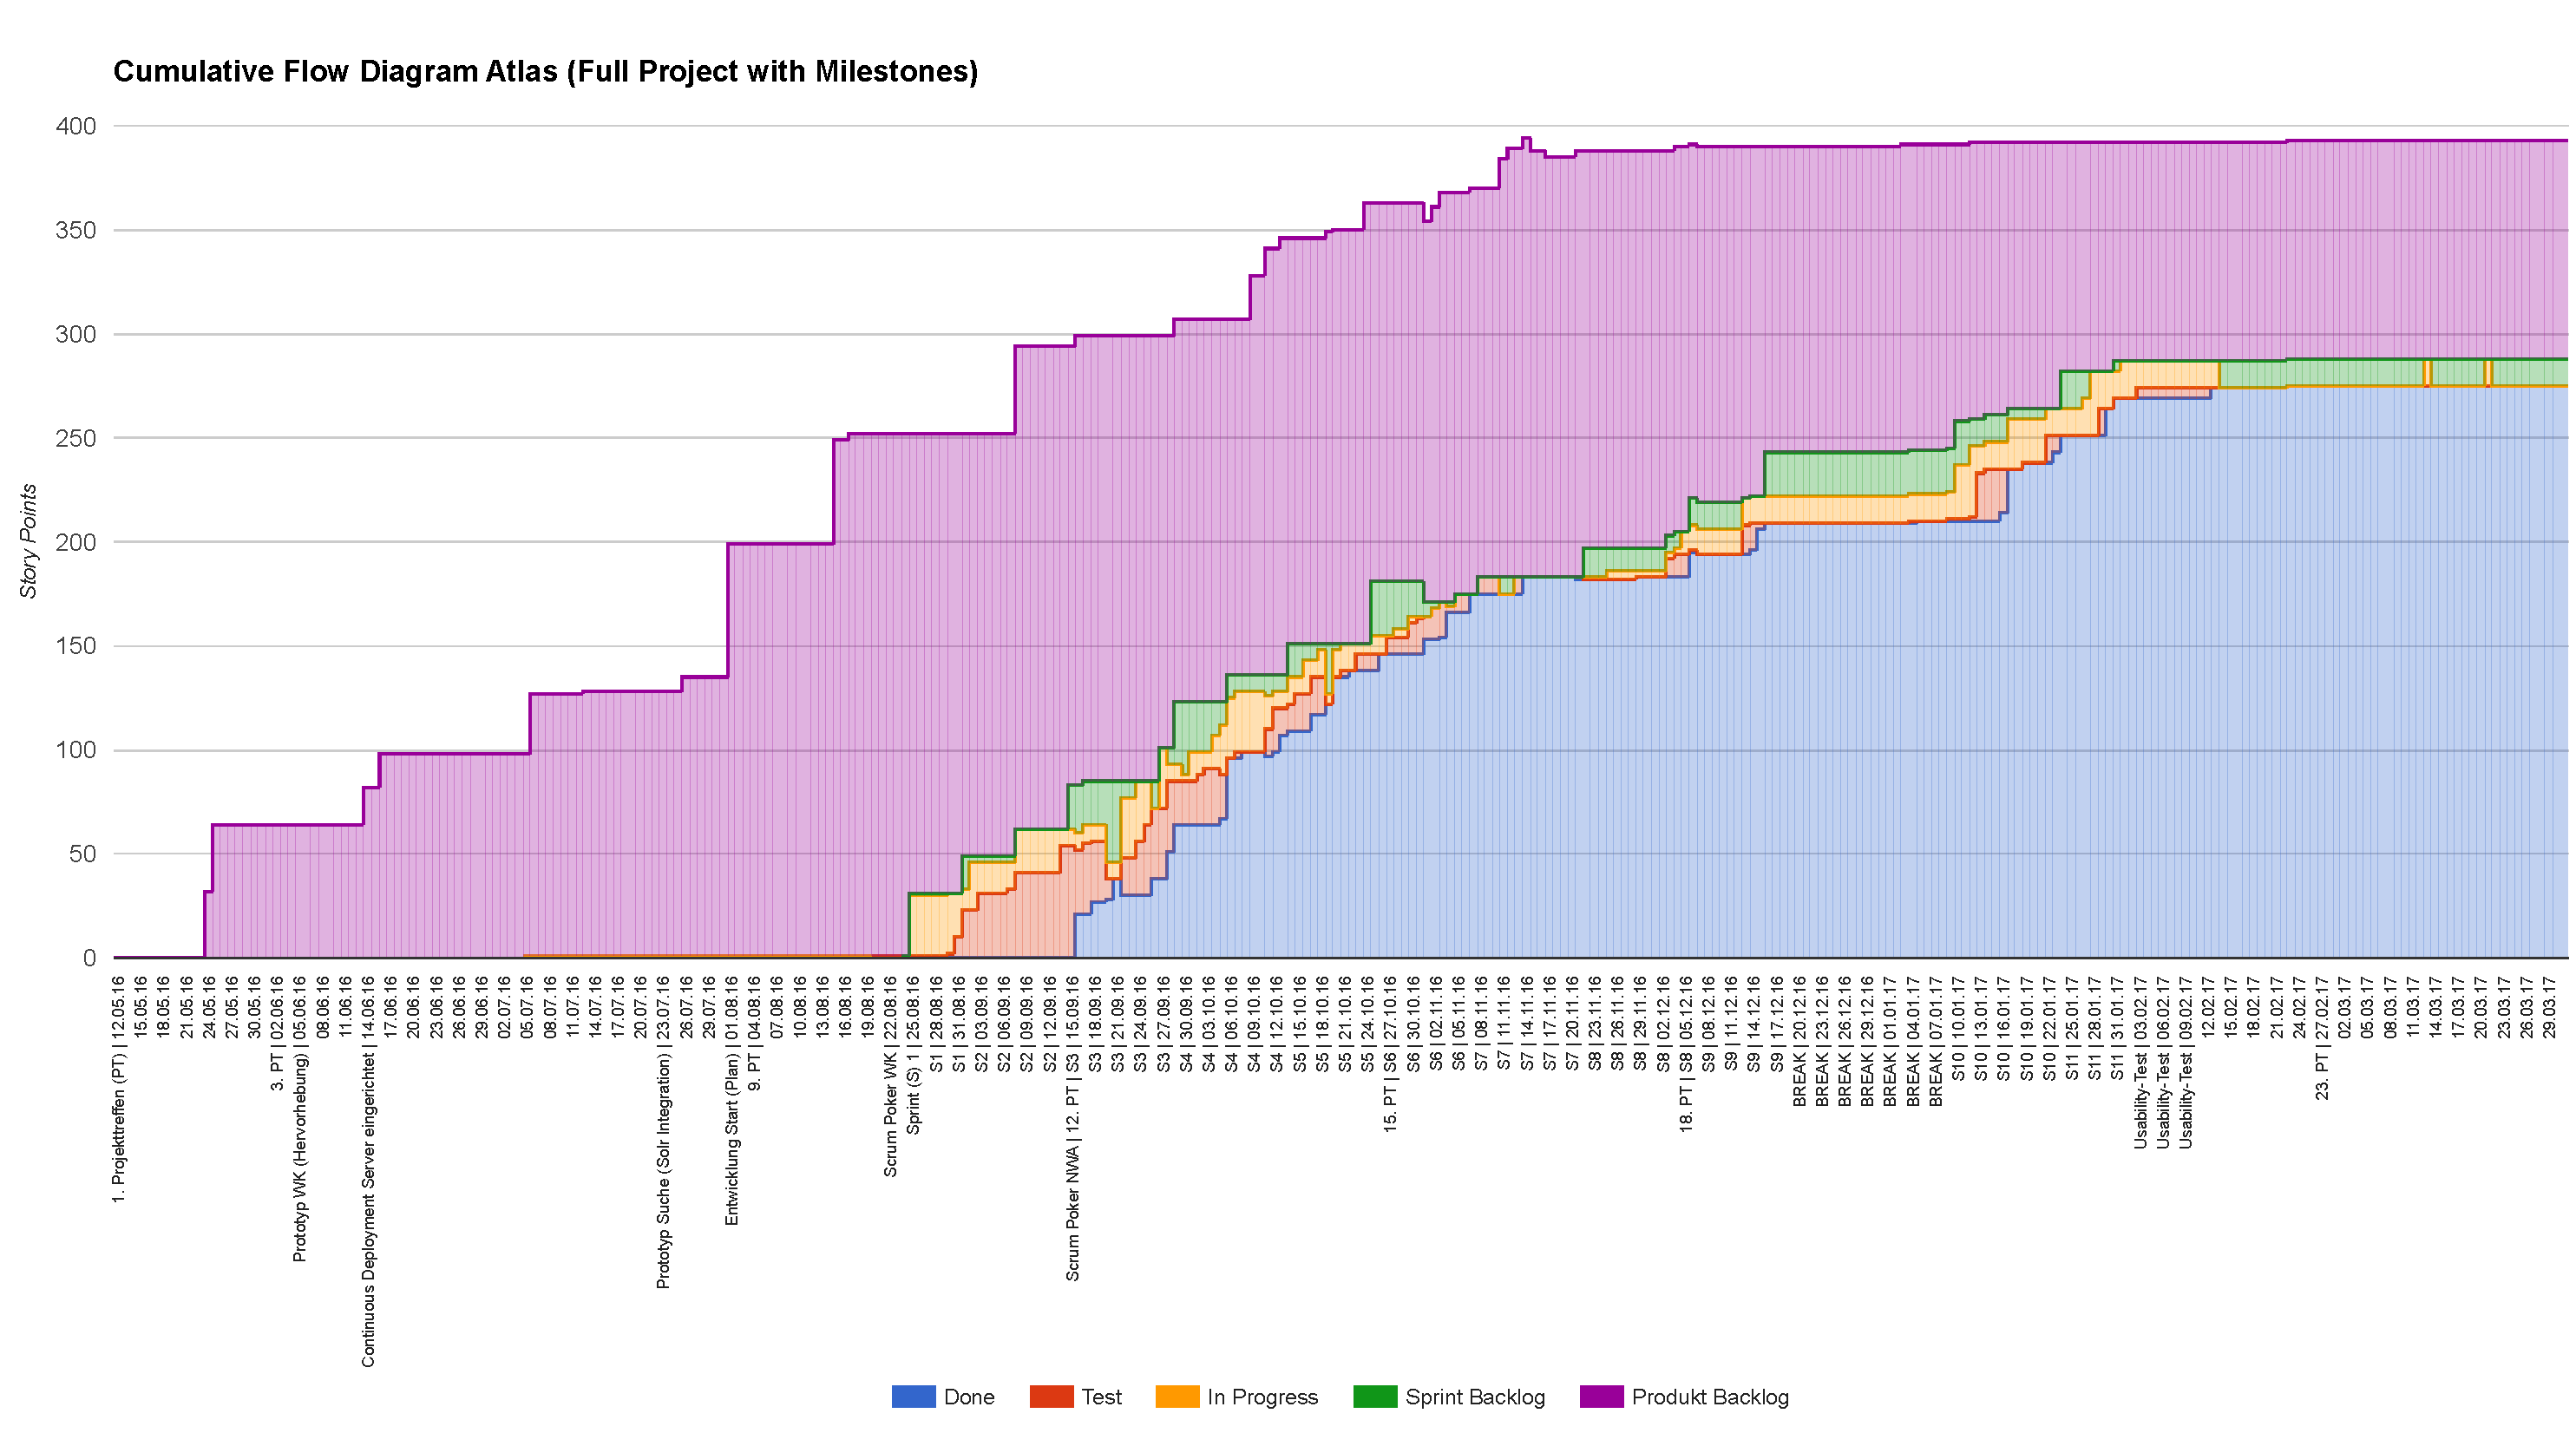
\includegraphics[page=1,width=\dimexpr\linewidth-2\fboxsep-2\fboxrule\relax]{svg/cfd_all}
		
		\vfill	
	}
	\captionof{figure}{\textit{Cumulative Flow Diagram} mit Meilensteinen (Gesamtes Projekt)}
\end{landscape}





\label{cfd_1st}
\pdfbookmark[1]{Cumulative Flow Diagram mit Meilensteinen (SoSe 2016)}{cfd_1st}
\begin{landscape}
	\parbox[c][\textwidth][s]{\linewidth}{%
		\vfill
		\captionsetup{type=figure}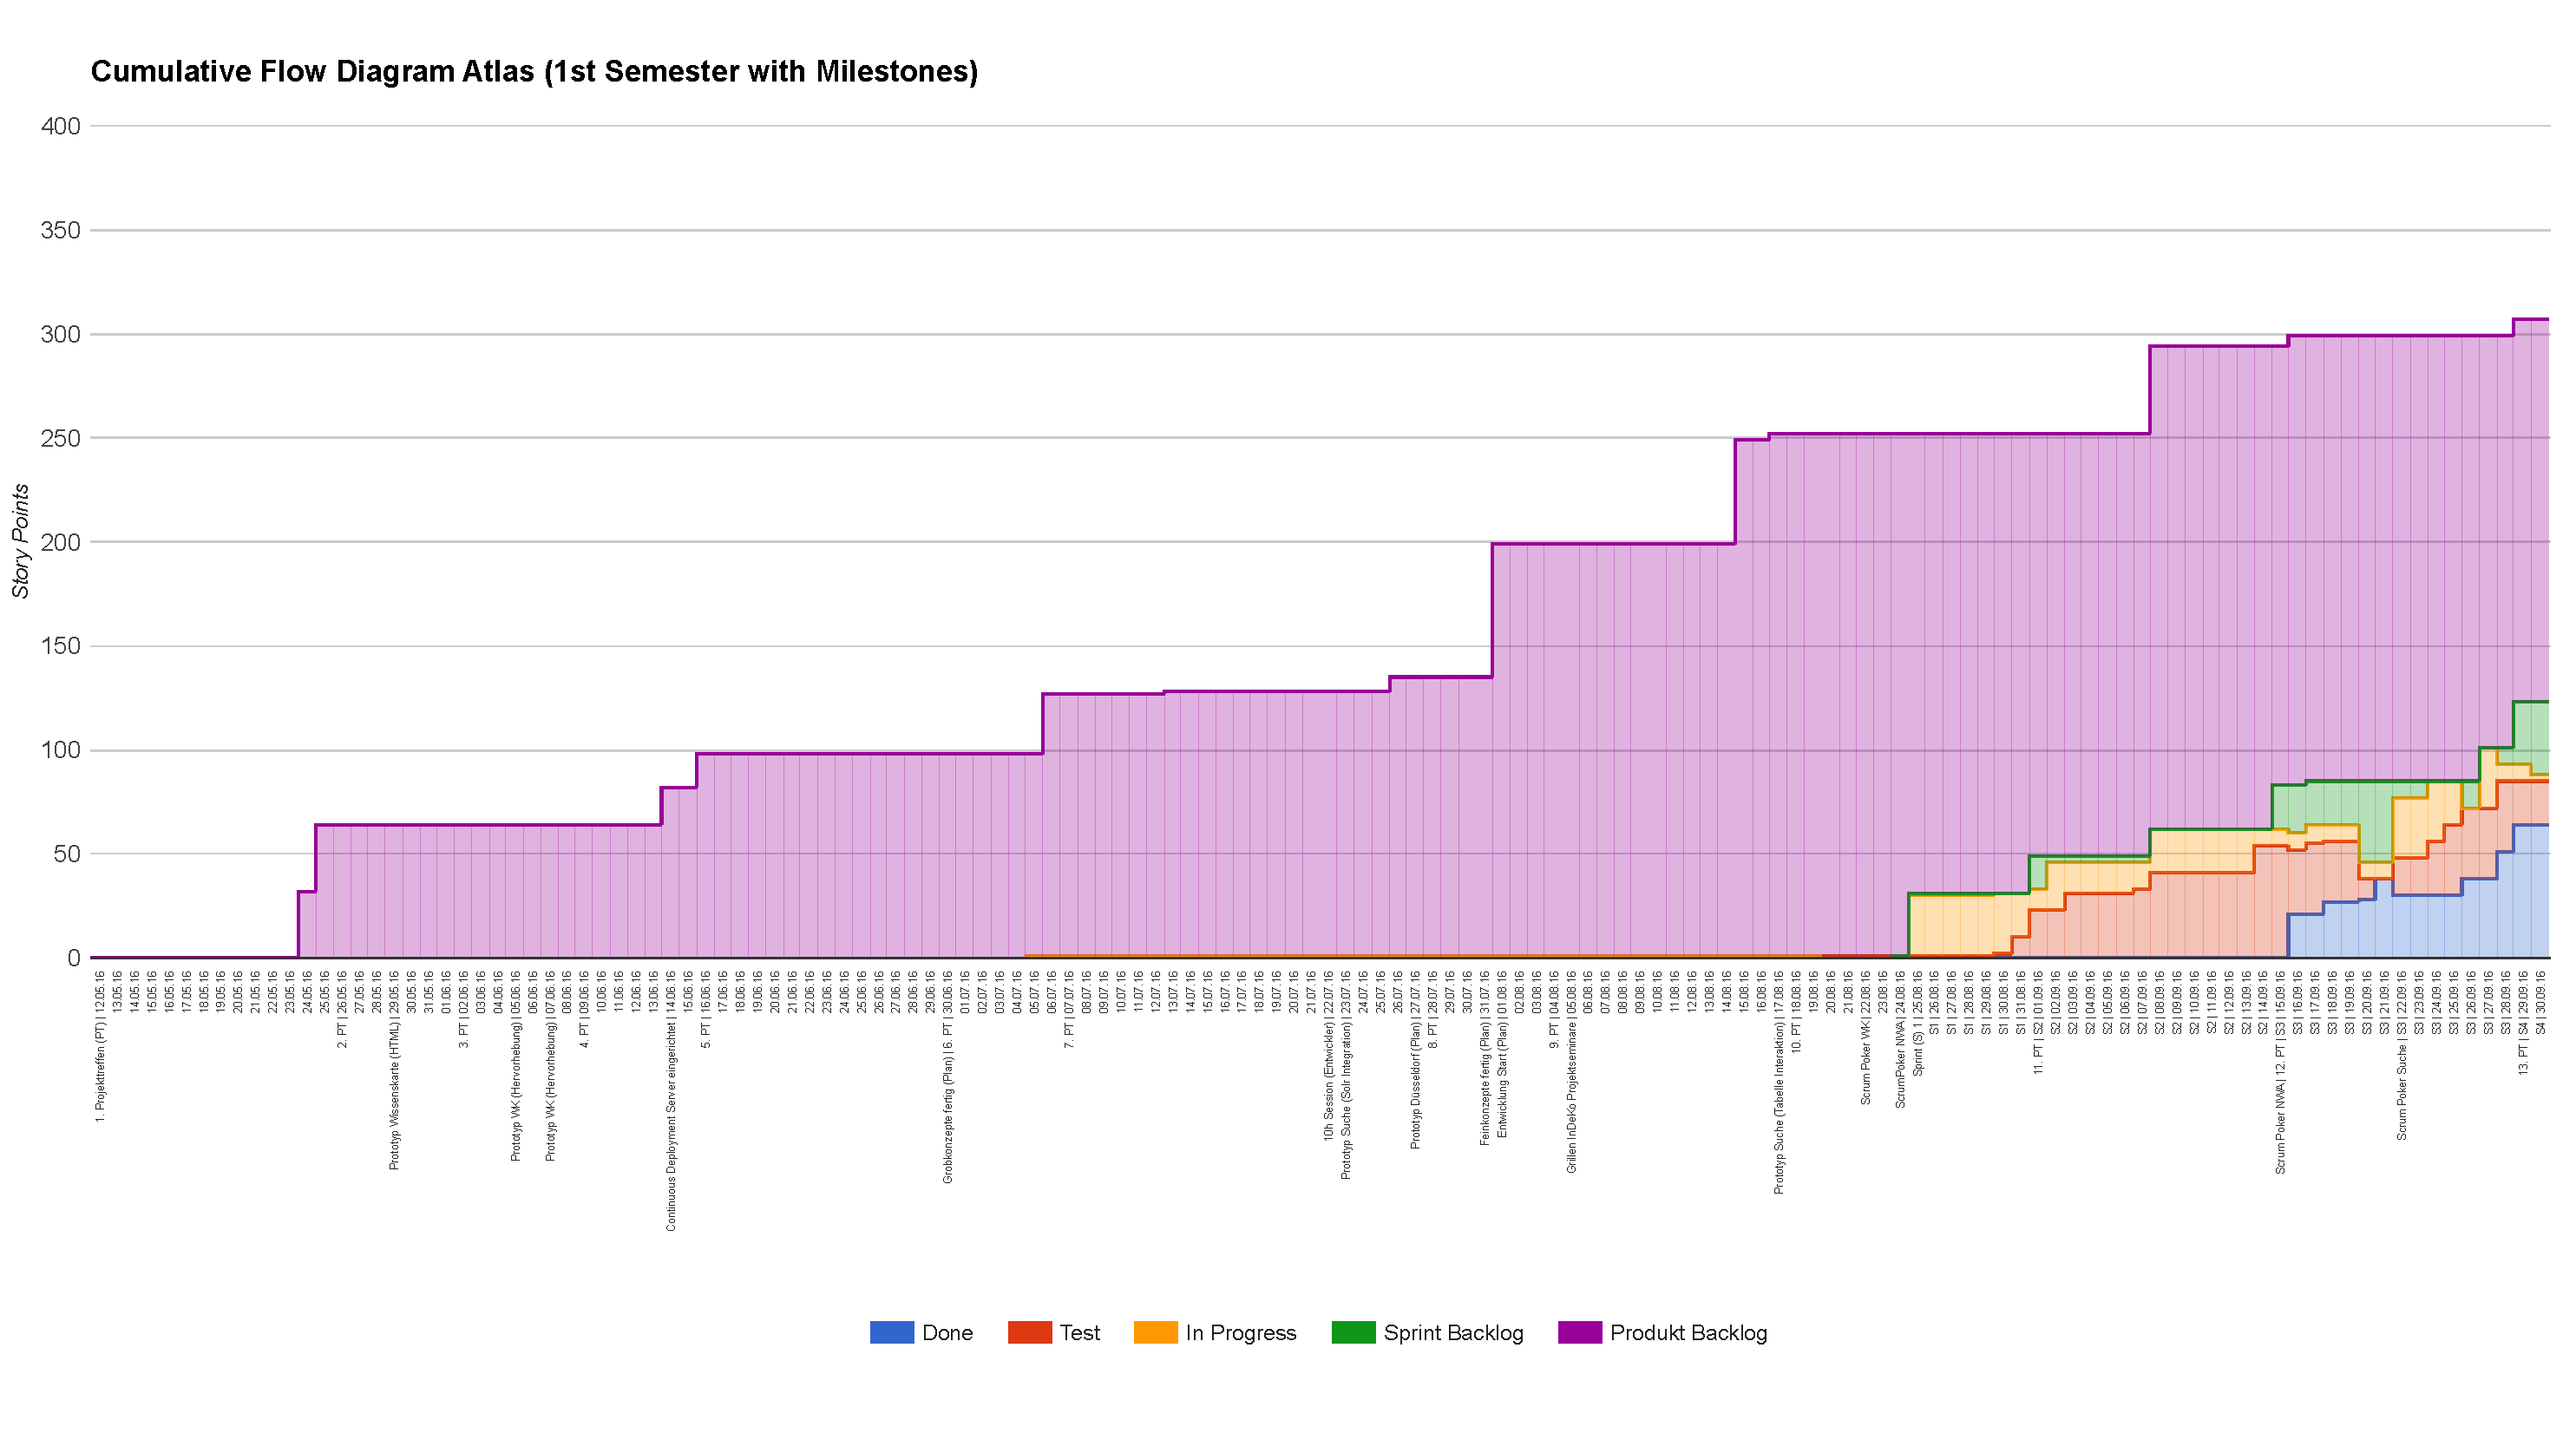
\includegraphics[page=1,width=\dimexpr\linewidth-2\fboxsep-2\fboxrule\relax]{svg/cfd_1st}
		
		\vfill	
	}
	\captionof{figure}{\textit{Cumulative Flow Diagram} mit Meilensteinen (SoSe 2016)}
\end{landscape}






\label{cfd_2nd}
\pdfbookmark[1]{Cumulative Flow Diagram mit Meilensteinen (WiSe 2016 / 2017)}{cfd_2nd}
\begin{landscape}
	\parbox[c][\textwidth][s]{\linewidth}{%
		\vfill
		\captionsetup{type=figure}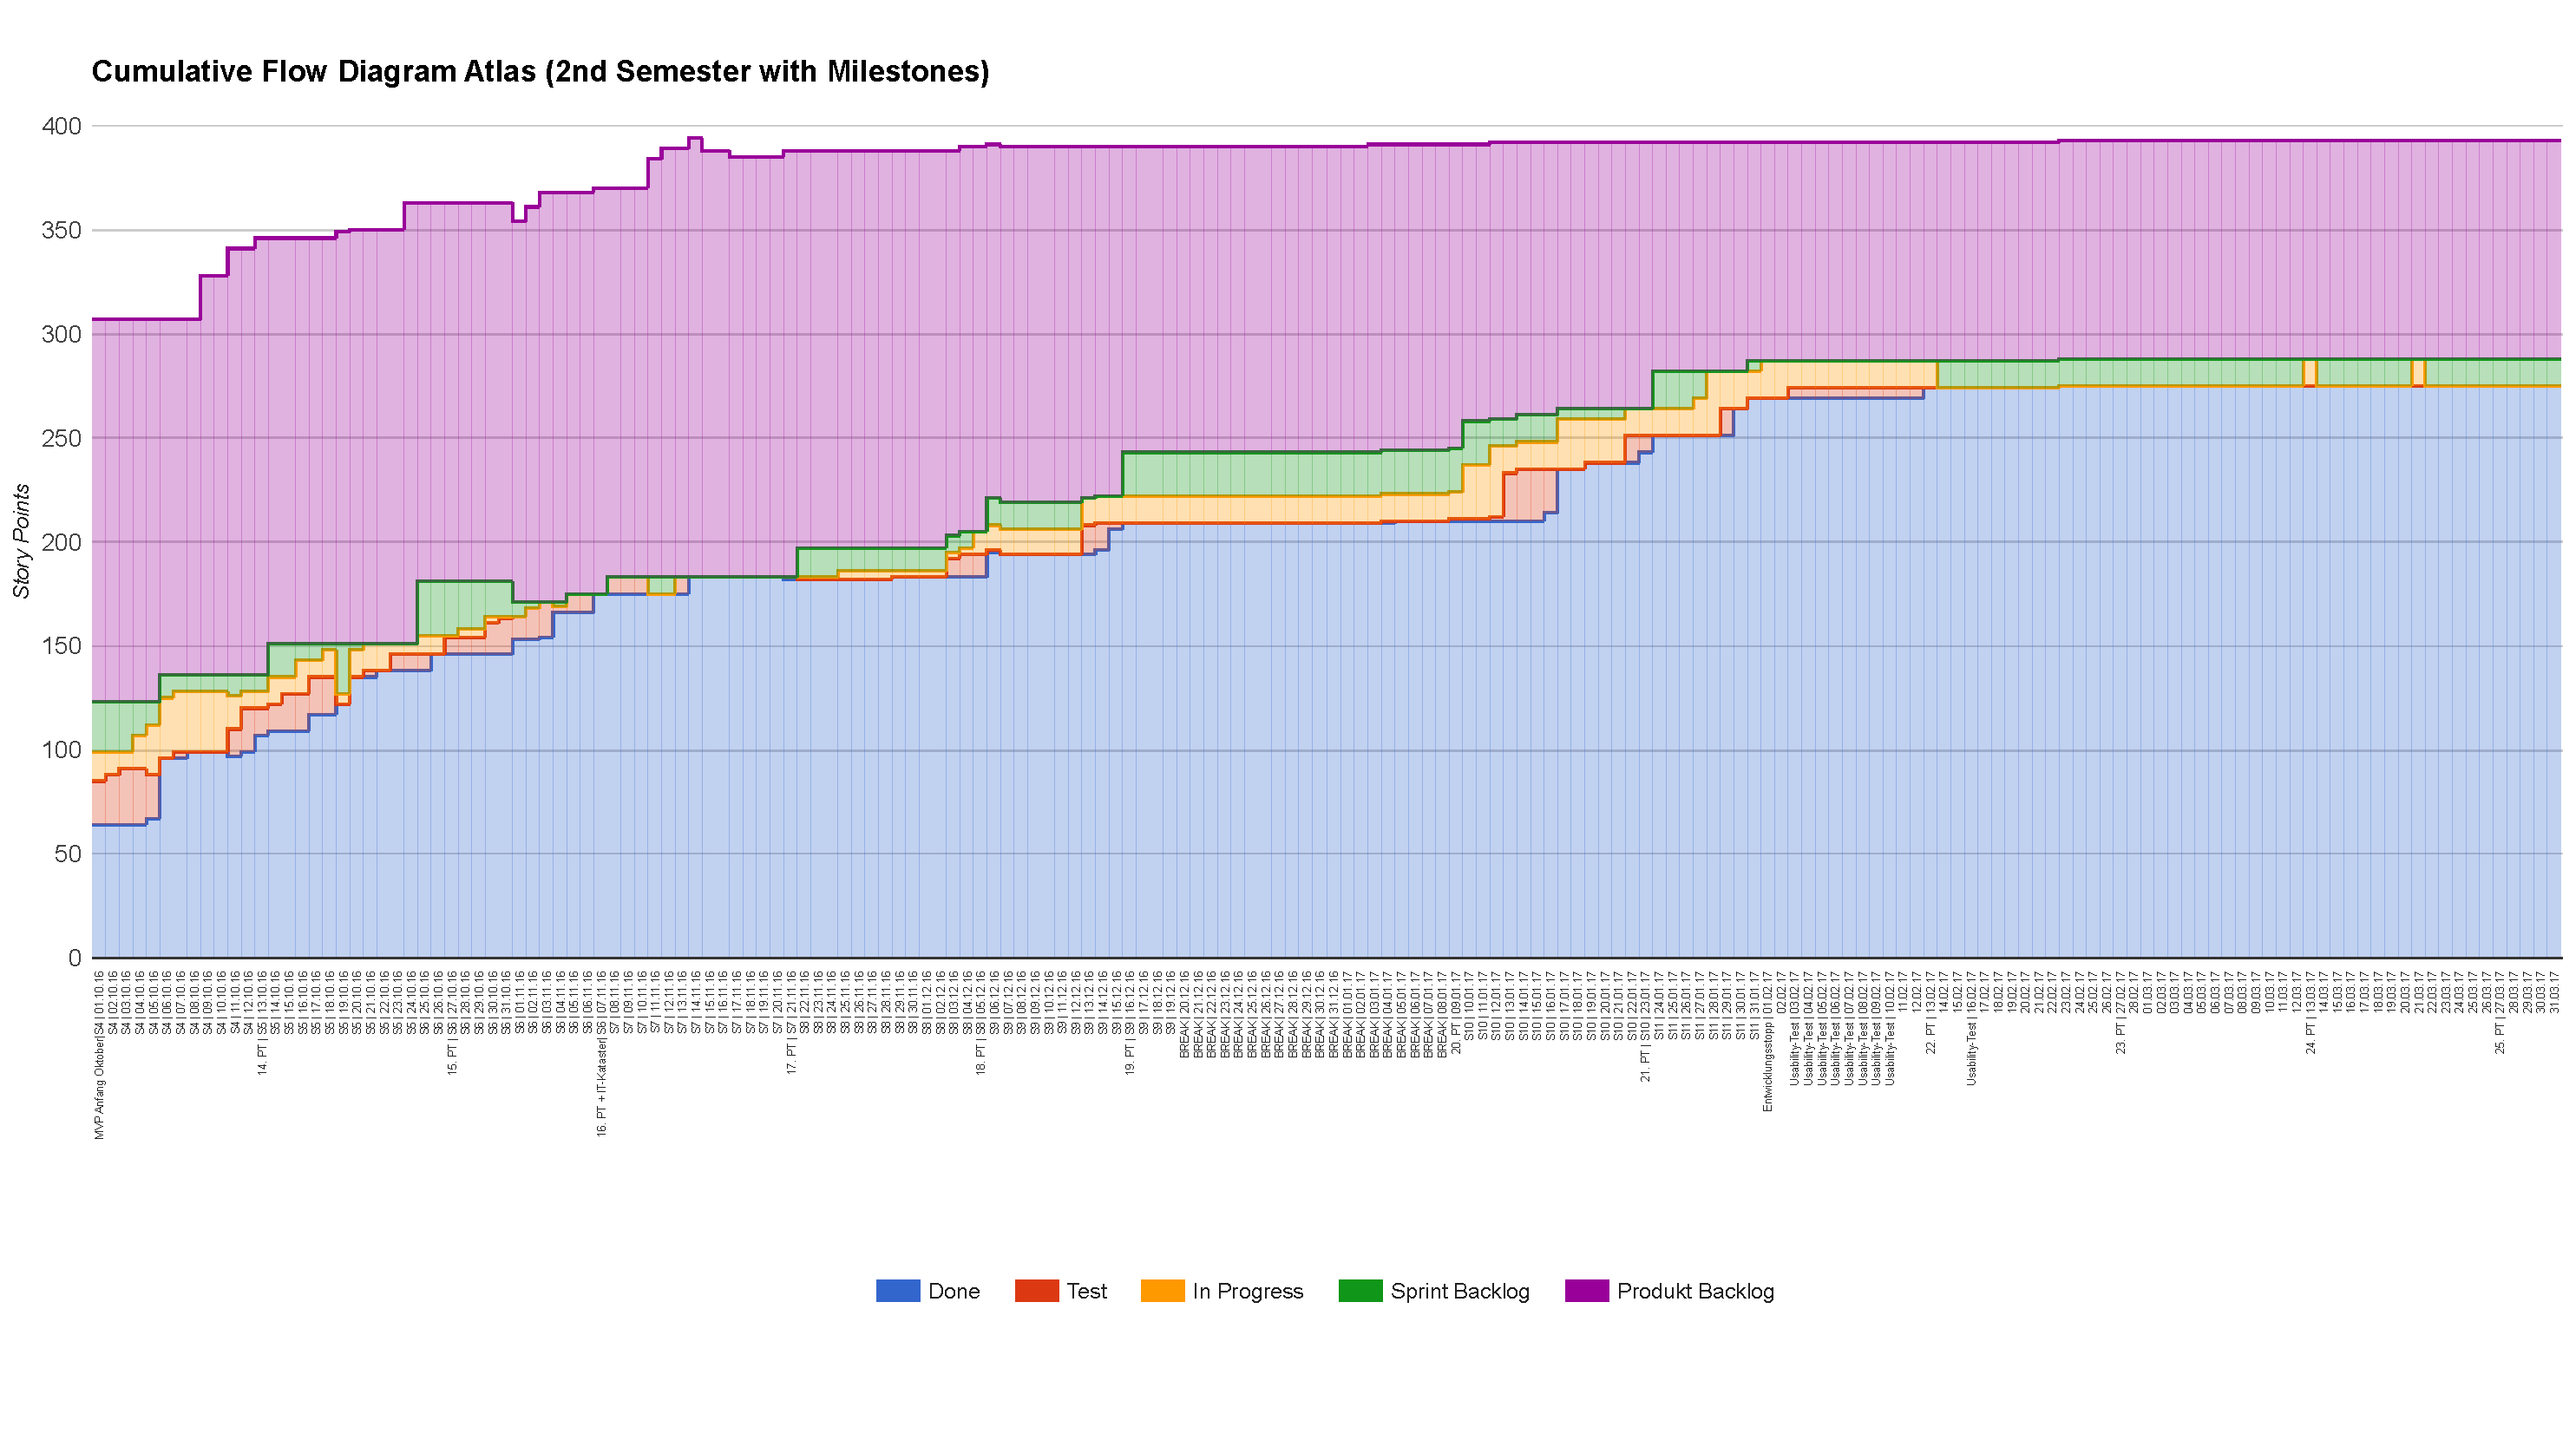
\includegraphics[page=1,width=\dimexpr\linewidth-2\fboxsep-2\fboxrule\relax]{svg/cfd_2nd}
		
		\vfill	
	}
	\captionof{figure}{\textit{Cumulative Flow Diagram} mit Meilensteinen (WiSe 2016 / 2017)}
\end{landscape}





\label{rohdaten_sprint}
\pdfbookmark[1]{Rohdaten (Sprintphase)}{rohdaten_sprint}
\begin{landscape}
	\parbox[c][\textwidth][s]{\linewidth}{%
		\vfill
		\captionsetup{type=figure}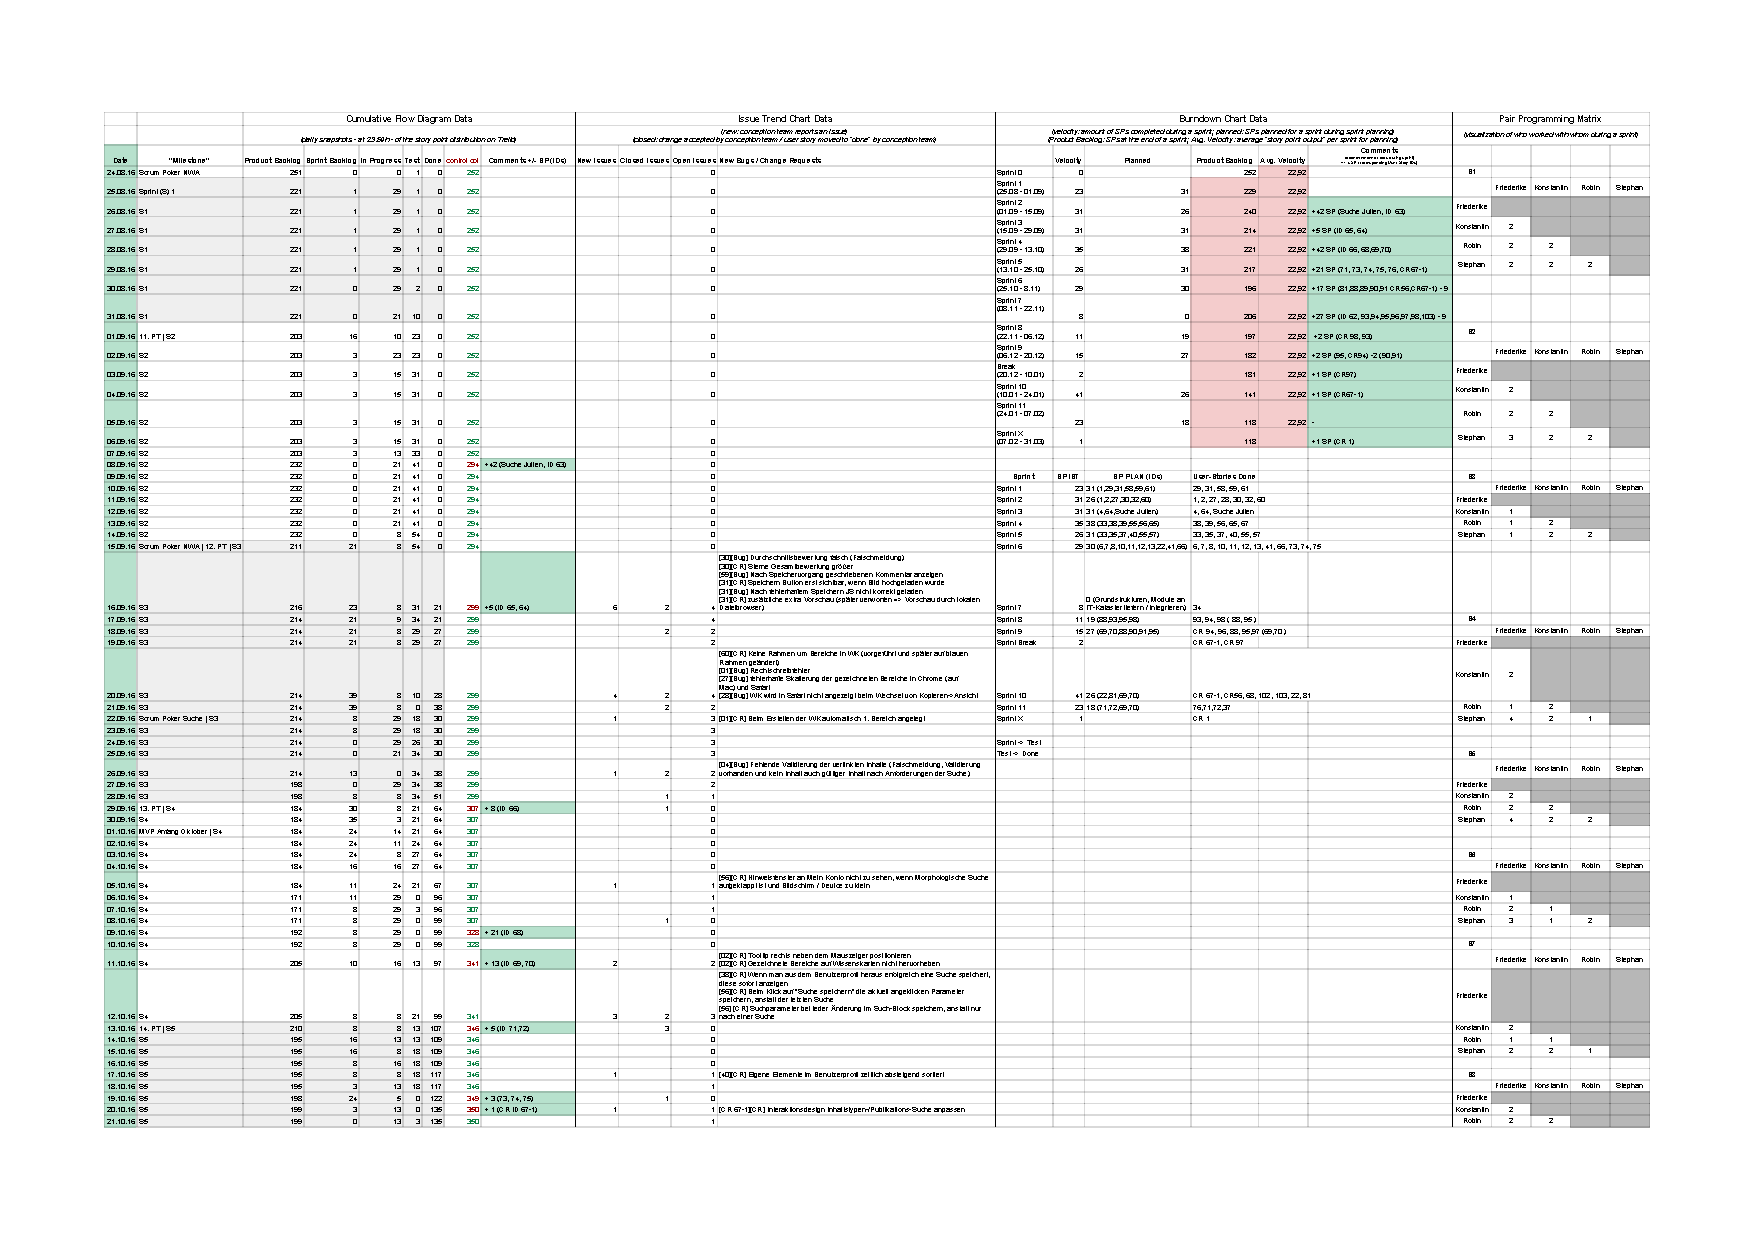
\includegraphics[page=1,width=\dimexpr\linewidth-2\fboxsep-2\fboxrule\relax]{data1}
		
		\vfill	
	}
	\captionof{table}[Rohdaten zur Überwachung und Steuerung 24.06.2016 - 21.10.2016]{Erfasste Rohdaten zur Überwachung und Steuerung der Entwicklung (Sprintphase) 24.06.2016 - 21.10.2016}
\end{landscape}

\begin{landscape}
	\parbox[c][\textwidth][s]{\linewidth}{%
		\vfill
		\captionsetup{type=figure}\includegraphics[page=2,width=\dimexpr\linewidth-2\fboxsep-2\fboxrule\relax]{data1}
		
		\vfill	
	}
	\captionof{table}[Rohdaten zur Überwachung und Steuerung 22.10.2016 - 04.01.2017]{Erfasste Rohdaten zur Überwachung und Steuerung der Entwicklung (Sprintphase) 22.10.2016 - 04.01.2017}
\end{landscape}

\begin{landscape}
	\parbox[c][\textwidth][s]{\linewidth}{%
		\vfill
		\captionsetup{type=figure}\includegraphics[page=3,width=\dimexpr\linewidth-2\fboxsep-2\fboxrule\relax]{data1}
		
		\vfill	
	}
	\captionof{table}[Rohdaten zur Überwachung und Steuerung 05.01.2017 - 31.03.2017]{Erfasste Rohdaten zur Überwachung und Steuerung der Entwicklung (Sprintphase) 05.01.2017 - 31.03.2017}
\end{landscape}





\newpage
\newgeometry{left=1cm,right=1cm,top=0cm,bottom=1cm,includefoot,footskip=0.5cm}
\resetHeadWidth
\setlength{\abovecaptionskip}{-30pt} % Chosen fairly arbitrarily




\begin{figure}
	\label{cfddataall}
	\pdfbookmark[1]{Cumulative Flow Diagram Daten}{cfddataall}
	\centering
	\captionsetup{type=table}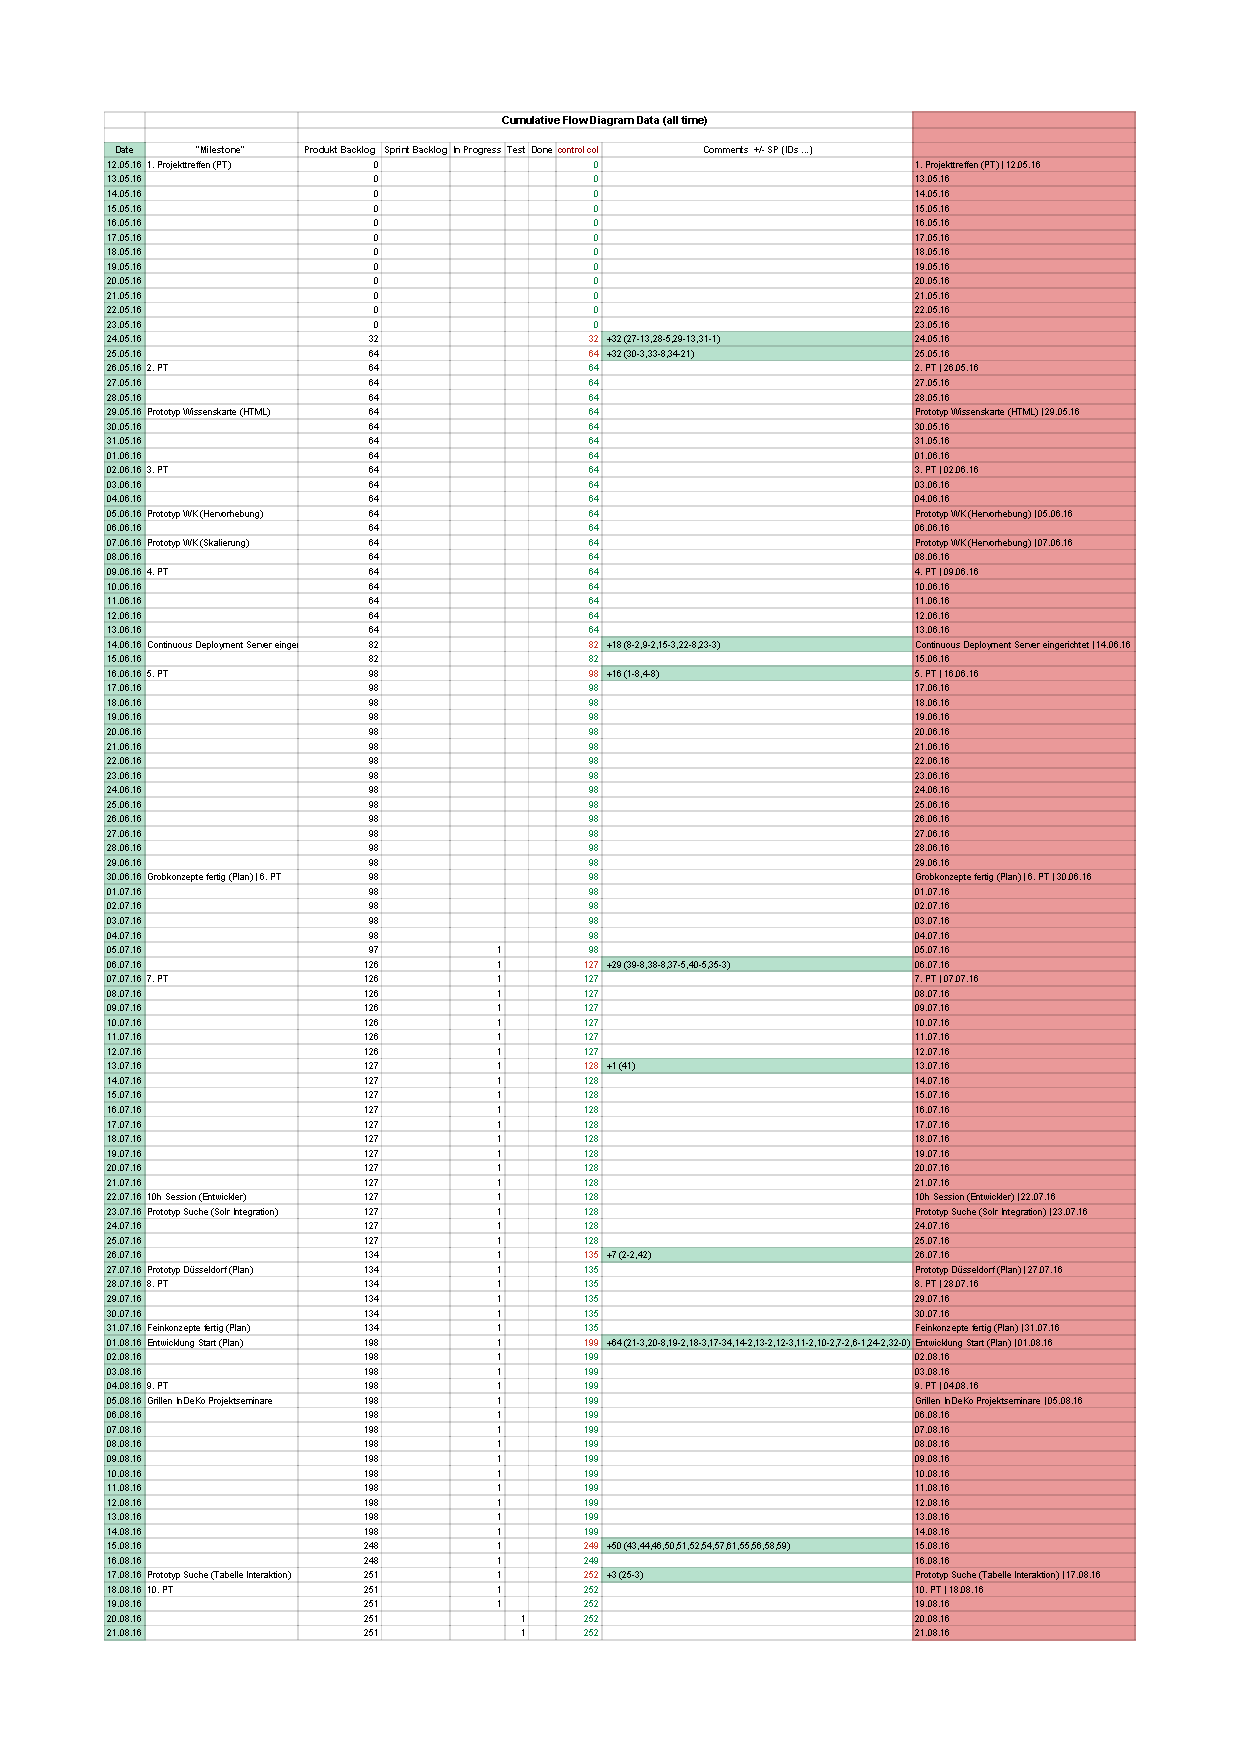
\includegraphics[page=1,width=\linewidth]{dataall}
	
	\caption{\textit{Cumulative Flow Diagram} Daten (Gesamtprojekt) 12.05.2016 - 21.08.2016}
\end{figure}
 
\begin{figure}
	\centering
	\captionsetup{type=table}\includegraphics[page=2,width=\linewidth]{dataall}
	\caption{\textit{Cumulative Flow Diagram} Daten (Gesamtprojekt) 22.08.2016 - 03.12.2016}
\end{figure}

\begin{figure}
	\centering
	\captionsetup{type=table}\includegraphics[page=3,width=\linewidth]{dataall}
	\caption{\textit{Cumulative Flow Diagram} Daten (Gesamtprojekt) 04.12.2016 - 18.03.2017}
\end{figure}

\begin{figure}
	\centering
	\captionsetup{type=table}\includegraphics[page=4,width=\linewidth]{dataall}
	\caption{\textit{Cumulative Flow Diagram} Daten (Gesamtprojekt) 19.03.2017 - 31.03.2017}
\end{figure}





\restoregeometry
\end{document}